\documentclass{article}
\usepackage[utf8]{inputenc}


\title{Appunti del corso di Economia dell'Innovazione - 2018/2019}
\author{Giulio Pilotto}
\date{May 2019}

\usepackage{natbib}
\usepackage{graphicx}
\usepackage{geometry}
\geometry{
	a4paper,
	total={170mm,257mm},
	left=20mm,
	top=20mm,
}

\begin{document}

\maketitle
\tableofcontents

\newpage
\section{Introduzione}
Il questo corso si esplorano due prospettive Economiche: quella dell'economia dell'innovazione che si interessa delle logiche per spiegare l'innovazione, e quella del management dell'innovazione che si occupa di studiare come metterla in pratica.


\textbf{NB} $\rightarrow$ Questi appunti contengono orrori ortografici e potrebbero non risultare completi. Chiunque voglia aggiornare questo documento può rivolgersi alla repo: https://github.com/giulio93/Economia\_Innovazione

 
\section{La teoria economica del valore}
Capire la natura della produzione permette alla politica economica di guidare l’economia su un percorso virtuoso di crescita economica (benessere economico).
Moderna confusione tra profitto (creazione) rendita
(estrazione) perché il concetto di valore oggi utilizzato
non ha un confine ben definito.
Oggi siamo incantati dal mito moderno della creazione
di valore ma se non distinguiamo tra creazione ed
estrazione rischiamo di remunerare di più la seconda
rispetto alla prima con conseguenze negative sulla
crescita economica (e la creazione di benessere)

\section{Le origini del concetto di valore}
\begin{itemize}
    \item Smith-Ricardo: Il valore è elemento critico per garantire la ri-produzione delle merci.
    \item Marx: Il valore
        partecipa alla definizione storica del metodo capitalistico di
        produzione.
    \item Neoclassici:  Il
valore c’è sempre stato e sempre ci sarà, indipendentemente dalla
forma dell’economia. 
\end{itemize}

La teoria economica comincia ad esistere in epoca borghese quando
il processo economico comincia ad essere dominato dal capitale. 
Per i fisiocratici diventa importante stabilire chi è produttivo e chi non lo è, e come si produce un intera economia.
Il concetto di \textbf{prodotto netto} diventa centrale: quella parte dell’intera
produzione sociale che eccede la ricostituzione sia dei mezzi di produzione, sia
dei mezzi di sussistenza necessari a coloro i quali, con il loro lavoro, hanno
portato all’esistenza della produzione stessa.
Con un esempio legato alla produzione agricola : il residuo che rimane dopo la riproduzione delle sementi le quali servono per garantire il processo economico, ossia lo scambio che crea mercato.



\begin{figure}[h!]
\centering
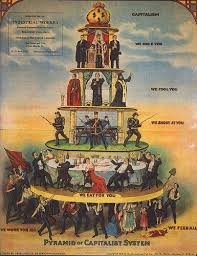
\includegraphics[scale=1.0]{images/fisiocratici.jpeg}
\caption{Pensiero Capitalista}
\label{fig:cap}
\end{figure}


\section{La scuola classica - dal valore nella terra al valore nel lavoro}
\begin{itemize}
    \item  la \textbf{rendita} è definibile come il reddito percepito in virtù della proprietà di una risorsa naturale scarsa o come la remunerazione eccedente il costo opportunità di un fattore produttivo.
    \item Il \textbf{profitto} (dalla lingua latina proficere: "andare oltre", "giovare") o lucro, in economia è l'utile (o "guadagno", indicato con G) che si ottiene da una certa attività economica (commerciale, finanziaria o produttiva).
\end{itemize}

\subsection{Smith -  prodotto netto composto da rendita e profitto}
Successivamente con l'industrializzazione della Gran Bretagna Smith arricchisce la definizione di prodotto netto come mero frutto della produzione e affermando che il valore di un bene dipende anche  a quanto lavoro serve per produrlo. 
Introduce cosi il concetto di \textbf{produttività}. Essa è legata alla divisione del lavoro quindi non dipende solo da una peculiarità del settore agricolo (la fertilità delle terre) ma dipende da caratteristiche
intrinseche al lavoro come tale, cioè dal lavoro in generale,
indipendentemente dai suoi campi d’impiego. 
\begin{figure}[h!]
\centering
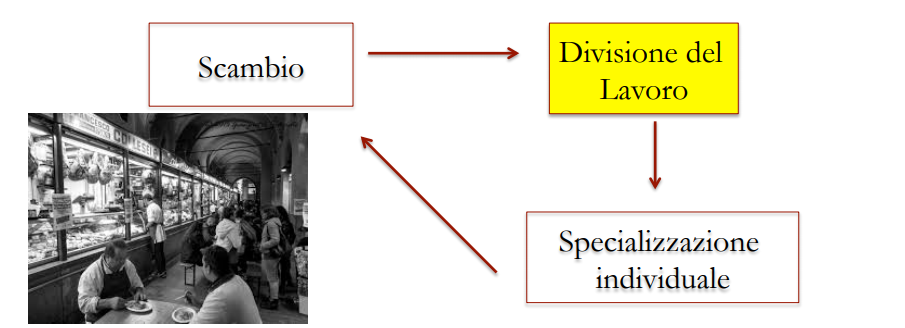
\includegraphics[scale=0.3]{images/spec_lav.png}
\caption{Smith: Mercato e prodotto}
\label{fig:spec_lav}
\end{figure}
Il \textbf{mercato} è il luogo della realizzazione degli scambi, dove cioè si ricostruisce il
nesso tra lavori individuali divisi e la reintroduzione degli uomini nella società
malgrado la specializzazione individuale.
La visione di Smith è centrata sui \textbf{rapporti sociali}. 
Il valore di scambio di una merce è il \textbf{prezzo reale}. Non il prezzo
monetario ma ciò che una merce  \textbf{realmente} vale. In origine il valore delle
merci è dato dalla quantità di lavoro necessaria a produrlo.
Per Smith, il valore della produzione non proviene da due fonti diverse (salari e
profitti) ma da un’unica fonte, il Lavoro.
\subsection{Ricardo - la distribuzione del lavoro}
Ricardo: Riprende la teoria del valore di Smith ma espande l’analisi ponendosi il problema di come il valore si distribuisce nella società sottolineando che la distribuzione non ha
nulla a che vedere con la formazione del valore. 
 Osserva il processo mercantilistico. Mette in evidenza come i processi di crescita economica non siano solo legati alla produzione, ma anche legati alla distribuzione della ricchezza nelle diverse classi sociali. Se la quantità di valore viene assorbito da una sola classe (aristocratici) ed essi hanno una rendita di valore (non producono) questo  è causa di stagnazione cioè di incapacità del sistema economico di riprodurre se stesso quando le rendite superano i profitti. 
Dibattito attuale: Le banche producono o non producono?

\subsection{Marx}
La teoria del valore in Marx ridefinisce il valore delle merci allo scopo di spiegare la
formazione del \textbf{plusvalore} non come residuo ma come reddito percepito dal
proprietario del capitale. La tesi fondamentale di Marx è che il lavoro è una merce
(fittizia) e ha un valore di mercato. Tuttavia l’oggetto dello scambio tra capitalista e
operaio non è il lavoro ma la sua capacità di lavorare \textbf{forza-lavoro}.
Per Marx il valore prodotto dall’operaio è maggiore del valore della sua forza-lavoro. 

\subsection{Verso una nuova teoria del valore - I Marginalisti}
Viene creata una visione “scientifica” del processo economico (produzione, scambio,
distribuzione del reddito).
 Sono chiamati cosi perche introducono la matematica nell' economia. Usano il calcolo infinitesimale per spiegare che succede al margine. Il valore per loro  è
 legato allo \textbf{scambio}, ovvero al mercato. Il valore dipende  dalla scarsita dei beni. Piu scarso e un bene (offerta), maggiore sara il prezzo, che definisce il valore. Il valore è soggettivo cioè è misurato dall’utilità per i \textbf{consumatore}.
Il valore viene correlato all’utilità. Rovesciamento della logica dei classici: il valore \textbf{basato sull’utilità} determina i costi di produzione e non il contrario, cioè i costi di produzione, inclusi i costi della manodopera, a determinare il valore.
Per i marginalisti, i mercati competitivi generano scambi di mercato a prezzi d’equilibrio e
quindi determinano esiti ottimali. Per ottenere esiti ottimali del processo capitalistico bisogna
eliminare tutti gli ostacoli e le imperfezioni del mercato. In questo quadro teorico la rendita
viene vista come un ostacolo (removibile) al buon funzionamento del mercato e non è più
“reddito non guadagnato”. 
\begin{itemize}
    \item In Ricardo valore = prezzo
    \item In Marx valore != prezzo (perché il valore deve essere trasformato in prezzo in quanto sono
categorie distinte. Marx usa il concetto di valore per rilevare le
contraddizioni del capitalismo).
\item Marginalisti Prezzo = utilità definita dai compratori 
\end{itemize}

\begin{itemize}
    \item Nell’economia \textbf{Classica} la rendita è l’equivalente del reddito da risorse scarse non prodotte
(ad esempio: i brevetti, le attività di corporazioni sociali come gli avvocati, le proprietà
fondiarie). La rendita, per utilizzare le parole di Marx è un diritto sul plusvalore sociale
complessivo.
\item Nell’economia \textbf{Neoclassica} i redditi corrispondono alla produttività. Non c’è rendita
(possibilità di guadagno a fronte di nessuna produzione) e nemmeno innovazione.
Se il prezzo definisce il valore dei beni allora il reddito che deriva dalla rendita è produttivo.
Non esiste, in questo quadro teorico, la categoria di reddito non guadagnato. 
\end{itemize}

Questo porta come conseguenza alla perdita del concetto di rendita.
Al giorno d'oggi per monitorare la ricchezza utilizziamo il Prodotto Interno Lordo.
In macroeconomia il prodotto interno lordo (abbreviato PIL) misura il valore aggregato, a prezzi di mercato, di tutti i beni e i servizi finali (cioè destinati al consumo) prodotti sul territorio di un Paese in un dato periodo di tempo (normalmente si usa come riferimento l’anno ma anche altri archi temporali sono usati).
Il PIL  è stato standardizzato negli anni 50. Misura la ricchezza ed e importante la decisione di cosa entra nella
misura del PIL:questa e una decisione a tavolino. 
\footnote{Riflessione sulla finanza: nella teoria  classica e neoclassica la  finanza si considerava  improduttiva, invece in questa fase attuale la finanza entra come misura importante. Le banche vengono considerate produttive.Il dibattito e comunque ancora aperto.}  

\section{Misurare la ricchezza}
I metodi contabili sono convenzioni sociali in evoluzione.
Non sono definiti da leggi fisiche e da “realtà” evidenti ma,
più semplicemente, riflettono le idee, teorie e ideologie
dell’epoca nella quale vengono sviluppati.Il PIL è influenzato dalla teoria del valore sottostante;
Il PIL è basato sul \textit{valore aggiunto} che esprime il valore
monetario di ciò che viene prodotto al netto del costo
delle materie prime o dei fattori di produzione intermedi 
Il \textbf{valore aggiunto} (anche abbreviato VA) in economia è la misura dell'incremento di valore che si verifica nell'ambito della produzione e distribuzione di beni e servizi finali grazie all'intervento dei fattori produttivi (capitale e lavoro) a partire da beni e risorse primarie iniziali.

Può essere calcolato:
\begin{itemize}
    \item dalla parte della produzione annuale
    \item dalla parte dei redditi (profitti , rendite e d interessi) annuali
    \item dalla parte della spesa, ricavata dalla domanda nei prodotti finali \footnote{Quali industrie aggiungono valore? Tutti i beni e servizi
che ricevono un prezzo sul mercato }

\end{itemize}


\section{Il concetto di Innvazione in economia}
L’aumento della produttività dei fattori è stato studiato anche dagli economisti
classici. 
\begin{itemize}
    \item \textbf{Smith}: studia “l’innovazione” come relazione tra
cambiamento tecnico, divisione del lavoro e cambiamento strutturale
dell’economia.
\item \textbf{Ricardo}: studia le conseguenze del progresso tecnico
incorporato nelle nuove macchine e distingue: effetti endogeni: la domanda aumenta perchè il prezzo delle macchine diminuisce, che ha un effetto sulla competizione tra imprese.
Effetti esogeni: la produzione di “innovazione”, cioè creazione di un
mercato di tecnologie e relativo impatto sull’occupazione. Lusso vs Beni primari.
\item \textbf{Marx} Per Marx il cambiamento tecnologico è un processo sociale nel senso che è il
risultato di una pressione competitiva e della dimensione del mercato (non è un risultato individuale)
\item \textbf{Schumpeter} Introduce il concetto di  \textbf{l'innovazione}.Il suo lavoro teorico è focalizzato sulla dinamica del cambiamento
 economico risultante dal processo di cambiamento tecnologico
di lungo periodo.
In un sistema capitalistico le imprese sono in competizione\footnote{La competizione tra le imprese è la leva all’accumulazione del capitale e alla crescita
della produttività. } e quello che dicevano i classici (Marx), è che il profitto ha una naturale decaduta per effetti di imitazione fra le imprese. Maggiore è il numero delle imprese, più aspra e la competizione e di conseguenza si ottiene una  riduzione dei prezzi e dei margini di profitto. Se la competizione cresce c'è una  caduta del saggio di profitti quindi  si attua ricerca di metodi per l aumento di produttività.
\end{itemize}
Gli elementi dello sviluppo per Schumpter:
\begin{itemize}
    \item \textbf{Innovazione}:distrugge i prodotti vecchi attraverso un processo di distruzione creatrice
    \item \textbf{L'imprenditore}:sviluppa progetti creativi affrontando il rischio, la resistenza al cambiamento e l'esitazione nel processo decisionale
    \item \textbf{Il credito finanziario}: : per introdurre un’innovazione è necessario controllare i mezzi di produzione (schei).
\end{itemize}
Per Schumpeter lo sviluppo economico ha bisogno del capitalismo come
istituzione. La competizione tecnologica determina l’evoluzione del capitalismo. 
Le imprese mantengono o migliorano la loro posizione competitiva attraverso aumenti
di produttività, cioè introducendo tecnologie più efficienti
In termini aggregati questo significa:
Accumulazione di capitale = aumento di produttività
La competizione per le tecnologie è la VERA competizione capitalistica, non quella
dei prezzi\footnote{Questo significa che ciò che veramente conta è “the competition from the new commodity, the
new technology, the new source of supply, the new type of organization, … (Schumpeter, 1943)}.
Conclusione: e condividiamo questa impostazione logica la conclusione e che le imprese competano per il prezzo, in realtà esse competono solo per avere vantaggi per le TECNOLOGIE. 

Invenzione per Schumpeter è una scoperta di nuova conoscenza. Non ha valore economico a priori. Rimane conoscenza finche non si individuta l utilita di quella tecnologia. Quado  entra nel mercato ed inventa\textbf{Innovazione}

\subsection{Cosa rende un impresa innovativa?}
Non esiste una definizione generale. Perché le caratteristiche di impresa innovativa
cambiano nel tempo. Spieghiamo questo punto.
L’impresa svolge un processo di trasformazione E dà vita a tre insiemi di attività a supporto dell’innovazione: strategiche, finanziarie , organizzative.
\begin{itemize}
    \item Le strategie d’impresa riguardano l’attività competitiva nei mercati dei
prodotti e le tecnologie da incorporare nel processo produttivo.
\item Le attività finanziarie riguardano gli investimenti necessari al cambiamento
tecnologico utile per accedere ai mercati (competitività tecnologica) e
riguardano la profittabilità attesa dell’investimento stesso.
\item Le attività organizzative riguardano la combinazione delle risorse per
ottenere un prodotto vendibile.

\end{itemize}
Queste attività hanno bisogno di un processo di apprendimento perché non è
affatto evidente come riuscire a produrre beni di buona qualità ad un prezzo
basso. 
Il processo di apprendimento è un’attività sociale, necessaria per l’innovazione.
Le sue caratteristiche sono: essere un’attività incerta, cumulativa e collettiva.

Pensiamo all’impresa innovativa: 
\begin{itemize}
    \item Deve differenziarsi dai competitors
    \item Trasformare la tecnologia e disturbare il mercato 
    \item Ridurre i costi dei prodotti già esistenti e al tempo stesso aumentarne la qualità.
\end{itemize}

\section{Le fonti dell'Innvoazione	}
\subsection{Caso PillCamera }

\begin{itemize}
	\item  \textbf{Problem Finding}: Nel 1981 Eitan Scapa, gastroenterologo israeliano convince GavrielIddan, ingegnere elettro-ottico che si occupava di controllo da remoto di missili,  a cercare una soluzione tecnologica più efficace di quelle a disposizione per esplorare il tratto interno dell’apparato digerente.
	\item  \textbf{Problem Setting}: Iddan si chiese se fosse possibile realizzare un dispositivo miniaturizzato a forma di missile senza che fosse collegato ad un cavo. Il dispositivo avrebbe avuto come “occhio” una telecamera. Problemi: qualità dell’immagine, durata batteria. (nel 1994 primo brevetto con la Applitec, ad Meron)  
	\item \textbf{Problem Solving}:  Nel 1997 Meron incontra  il dott. Swain direttore di un gruppo di ricerca in UK che stava lavorando ad un metodo di endoscopia wireless (a partire dalle microcamere disponibli sul mercato) usando frequenze a microonde. I due gruppi attivano una collaborazione e nel 1999 ottengono l’autorizzazione del comitato etico del RoyalLondonHospital per realizzare il primo esperimento su essere umano.
	Il gruppo inglese aveva una superiorità nel campo dell’anatomia umana e nella diagnostica per immagini dell’intestino mentre il gruppo israele-americano aveva conoscenze sula miniaturizzazione  dei dispositivi con basso assorbimento di energia. Nel 2001 il dispositivo ottiene il riconoscimento della FDA e GivenImaging viene quotata nella borsa NASDAQ dove raccoglie 60milioni di dollari nell’OPA iniziale.
\end{itemize}
Nasce PillCam, videocapsula da ingoiare con una piattaforma integrata (workstation, un software proprietario, una cintura da indossare con un sistema di videoregistrazione).
Fino al 2005 GivenImaging è \textbf{monopolista}. Nel 2005 Olympus introduce la sua telecamera in pillola. Altri gruppi di ricerca lavorano sul device (aggiungere gambe e pinze) GivenImaging si è \textbf{protetta} con un  patentthicket, contratti con  ospedali, corsi di formazione.

\subsection{Le fonti dell'innovazione}
Ne possiamo individuare principalmente alcune:
\begin{enumerate}
	\item \textbf{Individui}:
	\begin{itemize}
		\item \textbf{Inventore} ha una buona padronanza del settore in cui opera, che però potrebbe non
		essere l’unico campo in cui è specializzato. Tanto più l’oggetto sarà legato alla scienza e alla
		tecnologia, tanto più questo concetto è vero. L’inventore è curioso e interessato ai
		problemi; mette in discussione i modelli di pensiero dominanti (solitamente i grandi
		innovatori lo fanno).
		\item \textbf{Utilizzatore} possiede una profonda conoscenza dei propri bisogni e sono incentivati ad
		individuare soluzioni in grado di soddisfarli. Chi utilizza il bene ha
		una conoscenza superiore rispetto al suo produttore (es. snowboard). Le imprese devono
		tener conto delle potenzialità che possono provenire dagli utilizzatori.
		Le innovazioni ideate dagli utilizzatori possono anche far nascere nuovi settori come nel
		caso degli snowboard \footnote{I primi snowboard sono stati sviluppati da alcuni appassionati alla ricerca di nuovi  modi per sfrecciare sulla neve.Tom Sims realizzò il primo "ski board" in legno.Sherman Poppen creò uno "snurfer" nel tentativo di realizzare un giocattolo originale per sua figlia.Jake Burton aggiunse delle cinghie di gomma a strappo allo "snurfer" per averne un maggiore controllo.Oggi lo snowboard si è trasformato in un settore di grande rilievo, con milioni di praticanti sia in Nord America che in Europa.}.
	\end{itemize} 
	\item \textbf{Creatività di una organizzazione}:diversa perchè l'organizzazione ha delle caratteristiche sociali, che devono essere aderenti alla struttura organizzativa. Alcune sono più flessibili ed alcune più rigide.
	Al loro interno possiamo distinguere: singoli individui (es. dipendenti) e la funzione di
	Ricerca e Sviluppo (parte interna ala struttura organizzativa che svolge attività di sviluppo) \footnote{Il caso 3M (azienda americana produttrice di vari prodotti tra i quali il Post – It). Il Post – It
		nasce da un’invenzione di un dipendente dell’azienda. La 3M lavorava nel settore chimico
		come produttrice di colle, creò una colla particolare che venne usata da un suo dipendente
		per attaccare foglietti. Inizialmente il prodotto fu un insuccesso, i consumatori non ne
		capirono l’utilizzo. La 3M decise quindi di usare la strategia dell’opinion leader (influenza
		sui consumatori) regalando i post – it in luoghi pubblici per incentivare i consumatori. La
		3M è un’azienda nella quale i dipendenti hanno un tot di tempo di lavoro per fare ciò che
		vogliono; laddove individuino innovazioni verranno premiati}.
	
	\item \textbf{Relazioni  con  clienti,  fornitori, concorrenti o produttori  di  beni complementari } 
	\begin{itemize}
		\item Le relazioni di collaborazioneesterne stimolano le attività di R\&S, absorptive capacity.
		\item Le relazioni con l’Università ed enti di ricerca permettono di stare sulla frontiera tecnologica
		\item La ricerca con finanziamenti pubblici crea collegamenti tra il sistema delle imprese e il mondo della ricerca 
		\item La creazione di agenzie per il trasferimento tecnologico (parchi scientifici, incubatori) favoriscono l’accesso diretto all’esperienza scientifica (spin-off, start-up)
	\end{itemize}
\end{enumerate}

\subsection{Il ruolo della Ricerca}
\noindent
Tutti questi elementi specifici di individui e organizzazione definisco il problem setting e problem solving delle singole imprese. L'innovazione dipende dalla disponibilità di conoscienza, dall'ambiente in cui i soggetti agiscono e dalle capacita di apprendimento:pensare fuori dagli schemi aiuta a generare innovazione. Questa creatività si concretizza in disponibilità a investire in R\&S: più tutti sono innovation driven, maggiore sara disponibilità ad investire. come? con ricerca di base e ricerca applicata. la prima viene dall universita, la seconda e quando la ricerca e indirizzata a sviluppi di carattere economico.

\begin{itemize}
\item La ricerca di \textbf{Base o Pura}: essa consiste in processi orientati ad aumentare le
conoscenze dell’impresa senza considerare le applicazioni commerciali. Il suo
obiettivo è contribuire al progresso del sapere scientifico, che nel lungo termine
potrebbe poi offrire opportunità di mercato
\item La ricerca \textbf{Applicata} (effettuata sulla base delle conoscenze provenienti dalla
ricerca di base dell’impresa stessa o di soggetti esterni) è orientata all’aumento
della comprensione di un problema allo scopo di soddisfare un particolare bisogno. 
\item Per sviluppo si intende tutte le attività che consentono di applicare la conoscenza alla
realizzazione di nuovi prodotti, materiali o processi.
\textbf{Forte correlazione positiva tra quota di investimenti in R\&S di un’impresa e aumento nei ricavi e redditività}.
\end{itemize}



Ci sono due diversi approcci che l’impresa può assumere nei confronti di tale funzione:
\begin{itemize}
\item  \textbf{Science push}: in base al quale l’innovazione presenta un percorso
lineare che procede in sequenza dalla scoperta scientifica all’invenzione,
progettazione e quindi alle attività di produzione, fino ad arrivare al marketing.
Secondo questo approccio le fonti principali di innovazione sono le scoperte
scientifiche che vengono poi tradotte in applicazioni commerciali dall’impresa. La
funzione di marketing deve essere forte proprio perché il prodotto non viene
richiesto dai clienti.
\item \textbf{Demand Pull}: l’innovazione è guidata dalla domanda dei potenziali
utilizzatori, indirizzando l’impegno dei ricercatori dell’impresa verso lo sviluppo di
nuovi prodotti per cercare di rispondere ai suggerimenti o ai problemi del cliente.
\end{itemize}
La scelta tra i due approcci dipende sia dal settore in cui l'azienda opera, sia dalle dimensioni dell'azienda \footnote{In   Italia:   le   imprese   hanno   ancora   una   scarsa   propensione   agli investimenti  in  ricerca  (55,7\%  del  totale  investimenti  in  R\&D)  rispetto  al 67,5\% della Germania, all’84,5\% di Israele, 77,8\% di Giappone, 77,3\% di Cina e 70,6\% negli Stati Uniti}.

L'attività innovativa è condizionata da altri fattori:
\begin{itemize}
	\item I clienti 
	\item I fornitori \footnote{Un altro importante esempio di solida collaborazione con i fornitori italiani è UmbraGroup, che è diventata frontiere esclusivo di Boeing per le viti a ricircolo di sfere che sono installate su tutti i nostri aerei commerciali. Il Gruppo fornisce inoltre sistemi e componenti ad alta precisione con applicazione negli stessi velivoli. Nel tempo, il rapporto con Boeing ha consentito alla società di Foligno di espandersi negli USA, acquisendo una società di Seattle e aprendo una sua sede proprio in questa città.			}
	\item I concorrenti (processo di imitazione), imprese che operano nello stesso settore di riferimento.
	\item Imprese che appartengono ad altri settori produttivi.	
\end{itemize}

Spesso le imprese formano delle \textbf{alleanze} con clienti, fornitori, produttori di \textbf{beni complementari}
ed anche con i concorrenti per collaborare insieme ad un progetto di innovazione o per scambiarsi
informazioni ed altre risorse nella ricerca dell’innovazione.
Gli attori della collaborazione possono mettere in \textbf{comune risorse} quali il capitale e la conoscenza,
condividendo e distribuendo anche i rischi associati ai progetti di sviluppo di nuovi prodotti.
Le collaborazioni più frequenti coinvolgono le imprese e i propri clienti, fornitori o università locali.
Le fonti di innovazione possono essere interne (R\&S) o esterne (fornitori, altre imprese, ecc.).
La R\&S in house contribuisce a costruire la capacità di \textbf{assorbimento} dell’impresa, consentendo un
apprendimento e un utilizzo più efficaci della conoscenza acquisita da fonti esterne. La capacità di
assorbimento si riferisce all’attitudine dell’impresa a comprendere e impiegare nuove risorse di
conoscenza.
Ad oggi i grandi centri di ricerca esterni stanno sostituendo quelli interni.

\subsection{Network Collaborativi}
Il network collaborativo è un potente motore di innovazione . I network sono un
insieme di soggetti che hanno una qualche forma di legame e relazione tra di loro.
Comprende : Joint-venture, concessioni  di licenze, associazioni di ricerca, programmi, pubblico-privato, network informali.
La struttura della rete di collaborazione influenza  il flusso delle risorse , importante ruolo delle conoscenze e dell’informazione. 

I network collaborativi sono reti di imprese connesse tra loro e di istituzioni (università,
organizzazioni non profit, ecc.) operanti in determinati campi, concentrate territorialmente, dove
competono e allo stesso tempo cooperano, collegate da elementi di condivisione e di
complementarietà. La cooperazione può avvenire anche tra imprese concorrenti (es. Fiat e
Chrysler). Il concetto di network è diverso da quello di collaborazione in generale, poiché
quest’ultima prevede un \textbf{contratto lavorativo}.
Una forma di network sono i distretti industriali (es. Silicon Valley, Kilometro rosso a Milano), i
quali si contraddistinguono per le seguenti caratteristiche:

\begin{itemize}
	\item Divisione del lavoro tra imprese
	\item Condivisione delle informazioni
	\item Formazione e accumulazione di professionalità
	\item Sviluppo dei processi innovativi
\end{itemize}

\subsection{Concetto di Cluster Tecnologico}
Un altro esempio di network è il cluster tecnologico il quale è un insieme di aziende innovative che stimola la nascita di nuove imprese e attrae quelle esistenti, incentiva connessioni con fornitori e distributori sfruttando l'economia di prossimità infine attira competenze specializzate investendo in infrastrutture e servizi per la comunità.
I vantaggi di prossimità territoriale si chiamano \textbf{economie di agglomerazione}.
In essi è importante il fenomeno dello \textbf{spillover} tecnologico il quale si manifesta quando i benefici delle attività di
ricerca di un’impresa (o di altra istituzione, di un cluster o di una regione) si riversano su altre
imprese. Lo spillover tecnologico è un’azienda che nasce sulla base di una conoscenza sviluppata
da un’altra impresa; deve esserci un legame tra la base di conoscenza della nuova azienda con la
vecchia. I fattori che incidono sulla nascita degli spillover tecnologici sono:
\begin{enumerate}
	\item l’efficacia dei meccanismi di protezione della conoscenza (tanto meno ci sono meccanismi
	di protezione tanto più sarà facile prendere il know – how e creare spillover)
	\item grado di mobilità del capitale umano (possibilità di uscita dei lavoratori dalle aziende)
\end{enumerate}

\textbf{Attenzione}: La concentrazione territoriale genera anche effetti negativi 

\section{Forme e modelli dell'innvazione}

\subsection{Caso Studio Tesla Motor}
Macchina eletrica sportiva a basso impatto ambientale. Esisteva Toyota ma non era performante. incontra Musk. 
Tesla: progetto ardito (sfida al mercato automobilistico), superamento della fase della deathvalley, finanziariamente solida, capace di raggiungere gli obiettivi di mercato 

\subsection{Forme dell'innvoazione}
\begin{itemize}
	\item Innovazione di \textbf{prodotto} sono incorporate nei beni o servizi realizzati da un’impresa (Tesla Motor)
	\item Innovazione di \textbf{processo}: sono cambiamenti nelle modalità con le quali le imprese
	realizzano un determinato prodotto o servizio (es. tecniche di produzione, ecc.). Tali
	innovazioni sono spesso orientate al miglioramento dell’efficacia o dell’efficienza dei
	sistemi di produzione
\end{itemize}
Entrambe spesso sono innovazioni congiunte.
In base all’intensità e al grado di ampiezza distinguiamo (nella maggior parte dei casi si basa sulla
distanza dell’innovazione da un prodotto o da un processo preesistente):
\begin{itemize}
	\item innovazioni \textbf{radicali}: esse presentano un carattere di novità assoluta e devono
	risultare differenti in modo significativo dai prodotti e dai processi produttivi già esistenti
	(es. primo elicottero; prodotti di telecomunicazione wireless).
	\item innovazioni \textbf{incrementali}: esse non presentano caratteristiche particolarmente nuove
	o originali, possono infatti già essere note all’interno dell’impresa o del settore e consistono in cambiamenti marginali o in lievi adattamenti di soluzioni preesistenti (es.	nuova configurazione di un telefono cellulare con o senza sportellino a protezione della tastiera; modifiche elicottero).
	\footnote{Il caso delle macchine fotografiche digitali di Kodak e Sony: attività rischiosa per Kodak con un patrimonio di conoscenze sui processi chimici della fotografia (ri-orientamento strategico dell’azienda) mentre Sony possiede una sviluppata conoscenza nell’elettronica  e nello specifico nella grafica e registrazione digitale.}
\end{itemize}

In base all’effetto esercitato sulle competenze possedute dall’impresa:
\begin{itemize}
	\item innovazione competence enhancing: sono tutte quelle innovazioni che consistono in un'evoluzione della base delle conoscenze preesistenti (s. microprocessori Intel, ogni
	generazione di microprocessori incorpora un’innovazione ma fa leva sul patrimonio di
	conoscenze di Intel)
	\item innvoazione competence destroying: le innovazioni sono tali se la nuova tecnologia
	non scaturisce dalle competenze già possedute o se addirittura le rende inadeguate (es.
	passaggio dal regolo calcolatore alla calcolatrice tascabile; es. Polaroid, azienda produttrice
	di macchine fotografiche viene sostituita da un’azienda giapponese produttrice di
	macchine fotografiche digitali)
\end{itemize}

Solitamente le innovazioni competence enhancing sono sviluppate da imprese già operanti nel
settore; mentre le innovazioni competence destroying sono prodotte da imprese entranti nel
settore, ed esse sono generalmente innovazioni radicali e da queste possono nascere nuovi settori.
La maggior parte dei prodotti e dei processi è un sistema nidificato, ordinato in modo gerarchico.
La maggior parte dei prodotti e dei processi è un sistema nidificato, ordinato in modo gerarchico.
Ciò significa che l’entità considerata è un sistema di più componenti in cui, a sua volta, ciascun
componente consiste in un sistema formato da parti più piccole. Un’innovazione può implicare
una modifica dei singoli componenti (moduli, che per funzionare hanno bisogno di “parlare” la
stessa lingua e questo è possibile attraverso l’architettura), della struttura generale (architettura)
entro la quale operano i singoli componenti, o di entrambi. In base a ciò distinguiamo:
\begin{itemize}
	\item  innovazioni \textbf{modulari} prevede cambiamenti di uno o più componenti senza modifiche
	consistenti alla configurazione generale del sistema.
	\item innovazioni \textbf{architetturali} consiste in un cambiamento della struttura generale del
	sistema o del modo in cui i componenti interagiscono tra di loro.
\end{itemize}
In generale le innovazioni architetturali sono più importanti ed esse si ritengono di norma più
radicali e competence destroying (es. SYSTEM INTEGRATOR – sono aziende o specialisti che si
occupano dell’integrazione di sistemi e il loro compito è far dialogare impianti diversi tra di loro
allo scopo di creare una nuova struttura funzionale).
L’introduzione o l’adozione di un’innovazione modulare richiede all’impresa una conoscenza
limitata al componente oggetto della modifica; l’introduzione o l’adozione di un’innovazione
architetturale richiede una conoscenza più ampia dei meccanismi che governano le relazioni e le
interazioni tra le varie parti all’interno del sistema.

\section{Ciclo di vita di della tecnologia}
Le tecnologie hanno un loro sviluppo, una loro evoluzione e ciò prende il nome di traiettoria
tecnologica (l’insieme dei cambiamenti che avvengono negli anni).
Sia il tasso di miglioramento della performance di una tecnologia sia il suo tasso di diffusione nel
mercato tendono a seguire un andamento graficamente riproducibile con un curva a S.
Sebbene le due curve siano correlate fra loro (un miglioramento della performance può
incentivare ed accelerare la diffusione della tecnologia, mentre un maggior tasso di adozione può
sollecitare le imprese ad effettuare nuovi investimenti per mi

\begin{figure}[h!]
	\centering
	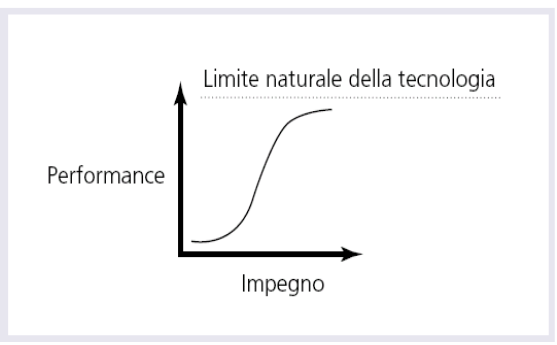
\includegraphics[scale=0.3]{images/curva_S.png}
	\caption{nella fase iniziale il miglioramento della performance è lento perché i principi di base della tecnologia sono stati compresi in maniera parziale. In seguito, quando aumenta la conoscenza della tecnologia, il miglioramento comincia ad essere più rapido. Infine, quando la tecnologia si avvicina al proprio limite naturale, la curva tende ad appiattirsi.}
	\label{fig:curva_S}
\end{figure}

Non sempre le tecnologie raggiungono il loro limite naturale.
Possono essere rimpiazzate da nuove tecnologie, definite, discontinue in quanto rispondono ad esigenze di mercato simili a quelle già soddisfatte da una tecnologia già esistente ma con una base di conoscenze completamente nuova.

\subsection{La diffusione della Tecnologia} 
Le curve a S sono usate anche per descrivere il processo di diffusione di una tecnologia. A
differenza delle curve a S della performance, le curve a S della diffusione di una tecnologia
esprimono il rapporto tra il numero complessivo di utilizzatori di una tecnologia (popolazione) e il
tempo.
In una fase iniziale, quando una tecnologia ancora poco conosciuta viene introdotta nel mercato,
l’adozione è lenta (i consumatori sono legati ad una precedente tecnologia); poi, quando gli
utilizzatori ne acquisiscono una comprensione maggiore, si diffonde nel mercato di massa facendo
aumentare il tasso di adozione (aumenta la capacità di performance della tecnologia e di
conseguenza la sua diffusione); infine quando il mercato tende a saturarsi il tasso di nuove
adozioni comincerà a diminuire.
Non sempre una nuova tecnologia si diffonde in modo veloce sebbene sia più performante della
vecchia tecnologia. Questo perché:
\begin{itemize}
	\item La nuova tecnologia potrebbe richiedere lo sviluppo di una complessa base di conoscenza;
	\item Molte tecnologie acquisiscono valore solo dopo lo sviluppo di una serie di risorse
	complementari
	\item Aspetti di carattere sociale, culturale e politico la rallentano (es. OGM)
\end{itemize}

I manager possono avvalersi dei modelli con curva a S per prevedere quando una tecnologia
raggiungerà i suoi limiti naturali, nonché affidarsi a tali modelli per decidere se e quando passare
ad una tecnologia innovativa o radicale.
Quale strumento di pianificazione la curva a S presenta però precisi limiti:
\begin{itemize}
	\item I limiti effettivi di una technolgia sono sconosciuti
	\item Cambiamenti inattesi del mercato, innovazioni nei componenti o nelle tecnologie
	complementari possono accorciare o allungare il ciclo di vita di una tecnologia.
\end{itemize}

\begin{figure}[h!]
	\centering
	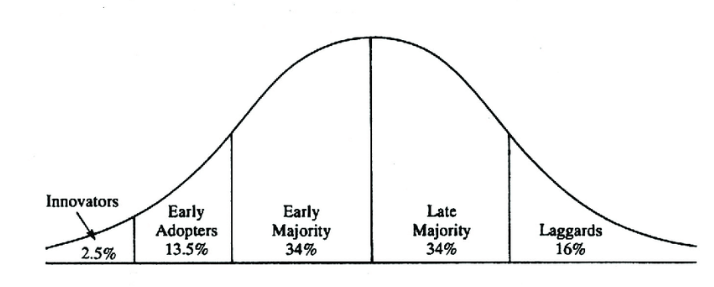
\includegraphics[scale=0.3]{images/adopters.png}
	\caption{Si studia analizzando il numero di utilizzatori di una tecnologia nel tempo}
	\label{fig:adopters}
\end{figure}

La fase di discontinuità tecnologica può modificare in maniera radicale la struttura competitiva di un settore industriale (Schumpeter distruzione creatrice).

\section{Conflitti di standard e disegno dominante}
\subsection{La concorrenza per lo standard dei pagamenti digitali}

Sqaure vs paypal
\begin{itemize}
	\item Convenienza
	\item Frode
	\item Ubiquità
\end{itemize}

Evoluzione: mobile banking

\subsection{L'affermazione di uno starndard dominante}
In breve: Diventare uno \textbf{standard} permette di sfruttare rendimenti crescenti di scala, ovvero all aumentare del volume di produzione i costi di produzione sono meno che proporzionali. Rendimenti crescente vuol dire anche che aumenta il numero di adottanti. A fronte di aumento dei profitti aumentano anche R\&S e l impresa investe anche in asset complementari. Rafforza anche cosi la posizione di cominanza della tecnologia. 

Il dominant design ha numerosi vantaggi, ma dall’altra parte porta alla perdita della
differenziazione (disomogeneità) poiché esse spinge verso l’omologazione. I fattori che portano
all’affermazione di un dominant design sono due:

\begin{enumerate}
	\item Fattori di tipo \textbf{istituzionale}: lo Stato fa una serie di interventi al fine di far affermare un
	dominant design (es. Tesla corrente alternata, UMTS nel settore della telefonia, ferrovie,
	ecc.).
	In determinati settori i benefici per il consumatore che derivano dalla compatibilità
	tecnologica degli standard sono tali da indurre gli organismi governativi a intervenire per
	imporre l’adesione ad uno standard tecnologico (es. politiche contro gli OMG in Europa).
	\item Fattori di natura \textbf{strategica}: In molti mercati le imprese convergono verso un unico disegno dominante. Uno dei motivi
	principali è che in tanti settori si manifestano rendimenti crescenti associati alla diffusione
	di una determinata tecnologia; quando cresce il numero degli adottanti, aumenta il valore
	della tecnologia.
	L’adozione e la diffusione di una tecnologia generano un margine di profitto che può essere
	reinvestito nello sviluppo e nel miglioramento della tecnologia stessa. L’utilizzo consente di
	acquisire una conoscenza più ampia e una più approfondita comprensione della tecnologia,
	permettendo di migliorare sia la tecnologia sia le sue applicazioni. Infine, un alto tasso di
	diffusione determina lo sviluppo di assets complementari concepiti per essere al servizio di
	quella tecnologia. Due fra le fonti dei rendimenti crescenti sono: effetti dell’apprendimento e
	esternalità di rete.
	
	\begin{itemize}
		\item \textbf{Effetti dell'apprendimento}  si hanno quando con l’accumulo di esperienza e di competenza
		tecnica, chi usa una determinata tecnologia impara a rendere il processo più efficiente, a
		volte sviluppando nuove soluzioni in grado di ridurre il costo degli input o l’impiego delle
		risorse utilizzate. 
		Esiste ampia evidenza empirica sulla correlazione positiva tra l’utilizzo di una tecnologia e il suo sviluppo, la sua efficacia e la sua efficienza.Questo fenomeno dell’apprendimento è rappresentabile dalla curva di apprendimento (o di esperienza), essa è una funzione del volume cumulato di produzione:
		la performance aumenta, o i costi di riducono, al crescere delle unità prodotte, solitamente
		con un tasso decrescente.
		L’economie di apprendimento ci dicono che l’utilizzo nel tempo di un bene porta ad una
		riduzione dei costi. Aumenta la performance della tecnologia con l’aumento della
		produzione.
		L’insieme di economie di apprendimento e aumento delle performance tecnologiche
		creano le basi per l’affermazione di un dominant design.
		C’è un binomio tra l’affermazione di un dominant design e la diffusione di una tecnologia
		(una tecnologia migliora la sua performance aumentando la sua diffusione).
		\item \textbf {Capacità di assorbimento} s’intende il processo di acquisizione di nuove conoscenze attraverso un’attività di apprendimento.Questo processo richiede: capacità di riconoscere valore a nuove informazioni e di saperle utilizzare in modo efficace. Ad esempio sperimentare non è una perdita di tempo in quanto si imparano procedure, organizzazione, necessità di competenze, ecc.Le imprese possono acquisire un vantaggio competitivo se per prime sperimentano e sviluppano nuove tecnologie. A livello aggregato: maggiore il numero di imprese che adottano e migliorano una tecnologia, maggiore sarà la capacità di assorbimento del sistema produttivo. E maggiori le tecnologie complementari che verranno introdotte per ulteriori miglioramenti di produttività
		\item \textbf{Esternalità della rete (o di consumo ) positive } si hanno ogni qualvolta il beneficio che deriva
		dall’utilizzo di un’innovazione aumenta al crescere del numero di utilizzatori. Aumentando
		il numero di utilizzatori della tecnologia aumenta il vantaggio (utilità). Se aumentando il
		numero di utilizzatori non aumenta l’utilità non si hanno esternalità di rete. Esse sono
		tipiche dei mercati basati su: reti fisiche (servizi ferroviari e telecomunicazioni), prodotti
		fortemente influenzati dalla presenza di beni complementari (beni accessori alla tecnologia
		legati ad essa) (Windows e le relative applicazioni software compatibili).
		Le CONOSCENZE COMPLEMENTARI (concetto diverso da bene complementare) sono legate
		allo sviluppo di un unico prodotto/tecnologia.
		È possibile rappresentare graficamente il valore offerto ai clienti da una nuova tecnologia
		considerando il valore generato dalle esternalità di rete.
		L’emergere di un dominant design fa nascere un problema di monopolio (presenza di leggi
		antitrust, le quali non condannano di per sé il monopolio, ma puniscono l’abuso di potere).
		I vantaggi di una situazione di monopolio sono dati dal fatto che esso porta maggiori profitti
		che l’impresa investirà in ReS.
		Il primo svantaggio per il consumatore, in una situazione di monopolio, è il prezzo troppo
		elevato per mancanza di concorrenza, altro svantaggio è che la qualità del prodotto non sempre è la migliore
	\end{itemize}
\end{enumerate}

\subsection{Formazione dei mercati winners-take-all}
Un’impresa in grado di affermare la propria tecnologia quale disegno dominante, di norma
guadagna enormi vantaggi e potrebbe riuscire a conservare la posizione dominante in quella
categoria di prodotto anche per il futuro. Quando un’impresa vede la sua tecnologia scelta come
disegno dominante non solo può cogliere l’opportunità di acquisire delle rendite di quasi-
monopolio nel breve termine, ma dispone anche della possibilità di “modellare” l’evoluzione del
settore e di esercitare una forte influenza sulle future generazioni di prodotto. Se un’impresa
sostiene una tecnologia che non è selezionata come standard del mercato, potrebbe esserecostretta a cedere il passo e a dover adottare la tecnologia diventata dominante, con una perdita
secca del capitale investito, dell’apprendimento e della reputazione di marca (brand equity). Nella
peggiore delle ipotesi, se non sarà in grado di adeguarsi alla tecnologia dominante, l’impresa potrà
persino essere estromessa dal mercato.
Gli economisti definiscono le arene competitive come mercati winner-takes-all (mercati in cui
predomina la tecnologia di un solo soggetto), dove il vincitore prende tutto.

\subsection{Valore stand-alone di una tecnologia}
Il valore (valore stand-alone) che una tecnologia offre ai clienti è determinato da una serie di
fattori:
Le funzioni d’uso che consente al fruitore di svolgere;
Il design e le sue qualità estetiche;
La semplicità di utilizzo.
Nei comportamenti d’acquisto dei consumatori non si considera solo la perfomance tecnologica
ma anche altri fattori.
Si deve tener conto della base di clienti, della presenza di beni complementari, ecc.
Nelle scelte strategiche delle imprese non si deve tenere conto solo della performance e dei limiti
della tecnologia ma anche di altre variabili.

\section{Tempo d'entrata}
La scelta del tempo d’ingresso (TIMING) con un nuovo prodotto in un mercato è una scelta
decisiva dal punto di vista strategico. Il timing sta assumendo sempre più importanza (modifica nei
gusti dei consumatori).
Ci sono tre diverse tipologie di strategia da poter adottare:
\begin{itemize}
	\item \textbf{First Mover} (primo entrante o pioniere) imprese che entrano per la prima volta nel
	mercato con un nuovo prodotto basato su competence destroying (innovazione
	radicale).
	\item \textbf{Early Follower} (primi inseguitori), sono imprese che entrano, successivamente, al
	first mover, ma ancora in una fase di incertezza (non si sa se il prodotto riuscirà ad
	affermarsi); il numero di imprese è maggiore rispetto ai first mover;
	\item \textbf{Late Entrant} (entranti ritardatari), imprese che entrano quando il prodotto o la
	tecnologia si è già affermata.
\end{itemize}

\subsection{Vantaggi di un First mover}
\begin{itemize}
\item Fedeltà di marca (brand loyalty), l’impresa guadagna una reputazione di lunga durata quale
leader in una determinata tecnologia. Tale status permette all’impresa di rafforza la sua
immagine, estendere la propria brand loyalty e allargare la quota di mercato anche dopo
l’introduzione di prodotti analoghi da parte dei concorrenti. Se le caratteristiche della
tecnologia sono difficili da imitare, la posizione di leadership tecnologica determina per
l’impresa una rendita da monopolio sostenibile nel tempo. Anche quando le caratteristiche
sono imitabili, il first mover ha comunque l’opportunità di costruire una relazione di fiducia
con il cliente prima dell’ingresso sul mercato dei concorrenti.
\item Diritto di opzione su risorse scarse (tutti i fattori necessari a sviluppare una certa
produzione, possono essere tangibili e non), le imprese che entrano per prime godono di
un vantaggio di prelazione o di opzione nell’acquisizione di risorse scarse. I concorrenti
potrebbero essere esclusi dall’accesso a tali risorse.
\item Sfruttamento switching cost dell’acquirente , una volta adottata una determinata
tecnologia il passaggio a una diversa comporta spesso dei costi per il cliente, definiti
switching cost. In particolare quando il prodotto è complesso, il cliente dovrà impegnare
parte del suo tempo per acquisire familiarità con esso. Tale investimento diventa uno
switching cost che scoraggia il potenziale acquirente dal passaggio a un prodotto
alternativo.
\item Vantaggi dei rendimenti crescenti , in un settore con pressioni competitive che spingono per
l’adozione di un progetto dominante, la scelta del timing degli investimenti nello sviluppo
di una nuova tecnologia può essere decisiva. Il first mover ha vantaggi (es. prezzo) poiché
avrà una massa di clienti superiore alle imprese che entrano successivamente.
\end{itemize}
Tutti questi vantaggi modificano la concorrenza tra first mover e imprese entranti
successivamente. L’importanza di tali vantaggi dipende dal settore di riferimento (es.
mercato della moda la brand loyalty è molto importante; nel caso di prodotto tecnologico
tale fattore non ha invece molta importanza).
\subsection {Svantaggi First Mover}
Esistono anche dei validi motivi per non entrare troppo presto in un mercato. Gli svantaggi del first
mover sono:
\begin{itemize}
\item Alti costi di ricerca e sviluppo , per essere leader nel settore l’impresa deve investire più
degli altri nella ReS. Il first mover per poter arrivare sul mercato con una determinata
tecnologia ha dovuto investire le proprie risorse in più progetti, poiché non sapeva quale
fosse la tecnologia migliore. I late entrant non devono investire in più progetti proprio
perché già sanno qual è la tecnologia su cui puntare.
\item Sviluppo dei canali di fornitura e distribuzione , tanto più il prodotto è innovativo tanto più
il first mover avrà difficoltà, non solo nella produzione, ma anche nella sua distribuzione al
cliente, per l’assenza o l’inadeguatezza del sistema di fornitori o distributori (es. Telecom,
first mover nella telefonia italiana)(es. Apple store, usato per la distribuzione hi-tech).
\item Sviluppo delle tecnologie abilitanti e dei beni complementari , le tecnologie abilitanti
servono per far funzionare la tecnologia principale (es. batteria dei cellulari).
\item Incertezza nelle condizioni della domanda , tanto più il prodotto è innovativo tanto più si
rischia il fallimento del prodotto (innovazioni di insuccesso) poiché non è detto che il
cliente lo capisca.
\item Incumbent inertia: i nuovi entranti sono in grado di adottare processi
produttivi più innovativi/superiore efficienza
\end{itemize}
Per quanto riguarda i follower (early follower e late entrant) i vantaggi del first mover sono loro
svantaggi; al contrario gli svantaggi del first mover sono i loro vantaggi.

\subsection{Fattori che determinano la strategia d’entrata ottimale}
\begin{itemize}
	\item Soddisfare una domanda già manifestata.
	Nella decisione il fattore discriminante sarà il rischio (gap tra rischio e benefici). Il fatto di
	sapere che cosa vuole il cliente abbassa il rischio di insuccesso. Tanto più il first mover
	immetterà sul mercato un prodotto che risponde alle esigenze del cliente tanto minore
	sarà l’incertezza e il rischio.
	\item Miglioramento rispetto alle soluzioni tecnologiche precedenti.
	Si ha nel caso in cui la nuova tecnologia soddisfa una domanda già esistente. Anche in
	questo caso il rischio è minore.
	\item Presenza di tecnologie abilitanti e di supporto.
	Se il first mover entra in mercati in cui ci sono già tecnologie abilitanti e di supporto il
	rischio è basso.
	\item Presenza di beni complementari (o di facile sviluppo).
	Se il valore dell’innovazione dipende dalla disponibilità e qualità dei beni complementari,
	saranno le caratteristiche di questi a determinare le probabilità di successo dell’entrata nel
	mercato. Se tali beni già esistono è più facile l’ingresso per il first mover.
\item 	Presenza di barriere all’entrata.
	La barriera all’entrata si ha quando la nuova entrante deve sostenere costi per entrare nel
	mercato maggiori delle imprese che già operano in esso. In una situazione di barriera
	all’entrata il first mover è incentivato ad entrare poiché ottiene un vantaggio rispetto ai
	follower (la barriera lo protegge dai concorrenti). È allo stesso tempo anche un rischio
	poiché il first mover deve sostenere elevati costi, laddove il prodotto non sia di successo ciò
	determinerebbe una perdita.
\item 	Presenza di rendimenti crescenti da adozione.
	Tanto più sono elevati i rendimenti crescenti tanti più conviene adottare una strategia di
	first mover.
\item 	Sostegno finanziario alle strategie di ingresso.
	Tanto più elevate sono le risorse finanziarie dell’impresa tanto più essa può sostenere il
	rischio.
\item 	Reputazione dell’impresa e incertezza del mercato.
	Oltre alle risorse finanziarie, anche la reputazione e la credibilità dell’impresa possono
	influenzare la scelta d’ingresso nel mercato. La reputazione dell’impresa invia forti segnali
	relativi alle possibilità di successo di una nuova tecnologia. Maggiore è la reputazione
	dell’impresa tanto minore sarà il rischio di insuccesso.
\end{itemize}

\begin{figure}[h!]
	\centering
	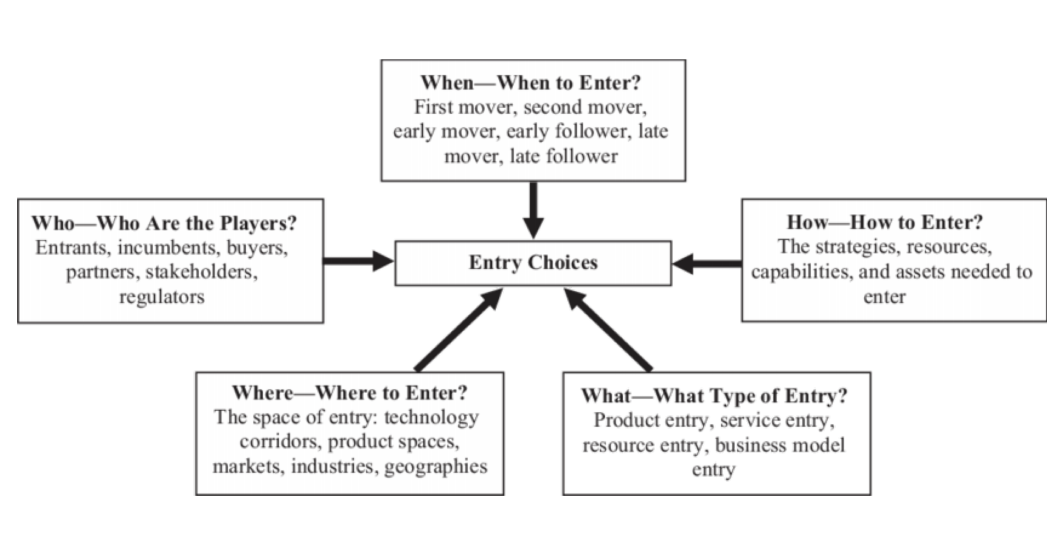
\includegraphics[scale=0.4]{images/Entry_choice.png}
	\caption{When you move first?}
	\label{fig:entry_choice}
\end{figure}

\subsection{First Movers vs Follower}
Se la tecnologia proposta dal first mover è performante ed è difendibile (alte barriere, bassa
imitabilità) conviene una strategia di first mover.
Se invece la tecnologia è incerta, facilmente imitabile e ci sono basse barriere all’entrata è
preferibile essere follower.
Sulla strategia da perseguire incide anche la dimensione e la disponibilità di risorse dell’impresa.
Già nella fase della ReS si può determinare la strategia d’ingresso. Le fasi della ReS sono:
Ricerca di base;
Ricerca applicata;
Sviluppo;
Capacità di assorbimento.
Se si decide di adottare una strategia di follower l’impresa investirà nella fase legata alla capacità
di assorbimento (la ricerca di base la prendi dal first mover e la inserisce nell’organizzazione).
Caso contrario, quando la strategia è di first mover, l’impresa investirà in ricerca di base.
È nella fase della progettazione della funzione di ReS che le imprese stabiliscono la strategia da
adottare.

\subsection 
{FMA nel mercato Abilitato da Internet}

\section{Definizione dell'orientamento strategico}
\subsection{Come si contruisce nua strategia basatas ull'innovazione?}
Per analizzare una strategia è necessario:Valutare la posizione competitiva dell’impresa,definire l’orientamento strategico per il futuro.
\begin{figure}[h!]
	\centering
	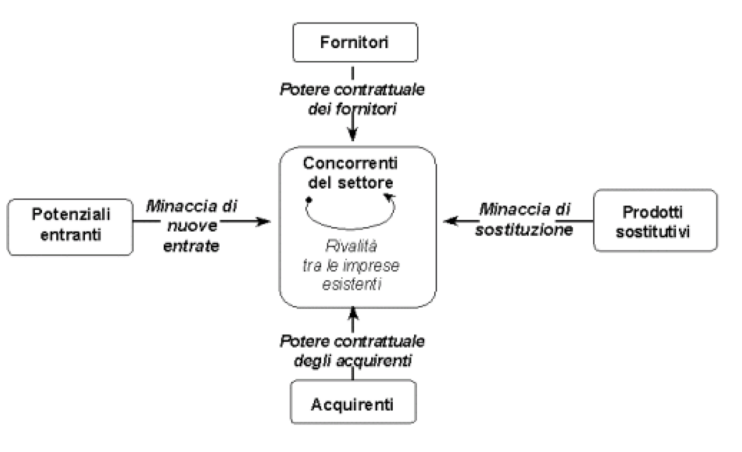
\includegraphics[scale=0.4]{images/Porter.png}
	\caption{Il modello delle cinque forze di Porter (1980)
		per la valutazione della posizione competitiva
		dell’impresa. Modello
		utilizzato per
		valutare:
		Attrattività di
		un settore e
		L’ambiente
		competitivo
		di un’impresa}
	\label{fig:Porter}
\end{figure}

Il grado di competitività  dipende:
\begin{itemize}
\item Numero e dimensioni dei concorrenti
\item Differenziazione dei concorrenti
\item Condizioni della domanda
\end{itemize}
Minaccia di entranti potenziali dipende:
\begin{itemize}
	\item Attrattività del settore (es. redditività)
	\item Barriere all’entrata (scoraggiano l’ingresso)
	\item Strategie di penetrazione (es. partnership)
\end{itemize}
Il potere contrattuale dei fornitori
dipende:
\begin{itemize}
	\item Numerosità dei fornitori
	\item Differenziazione dei fornitori
	\item Switching cost per passare ad un
	altro fornitore
	\item Integrazione verticale a monte da parte degli acquirenti
\end{itemize}

La minaccia dei prodotti sostitutivi:
\begin{itemize}
	\item Similarità della loro funzione con quella
	dell’impresa
	\item Prezzo relativo dei beni sostitutivi
\end{itemize}

Sesta forza: i beni complementari
La disponibilità, qualità, prezzo dei complementi
influenzano le opportunità e le minacce per le
imprese del settore.

\subsection{Analisi stakeholders}

\begin{figure}[h!]
	\centering
	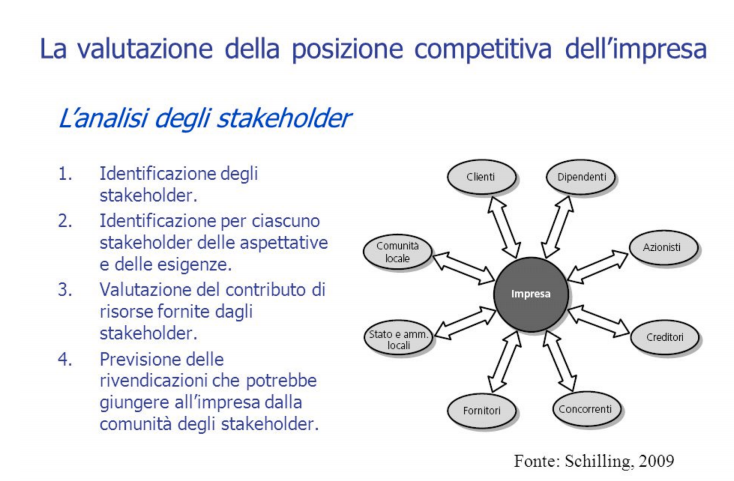
\includegraphics[scale=0.4]{images/stakeholders.png}
	\caption{Analisi stakeholders di Porter}
	\label{fig:Porter2}
\end{figure}

\subsection{Analisi del cambiamento interno }
Ciascuna attività può essere valutata in base alla sua capacità di contribuire alla creazione del valore complessivo dell’impresa Identificati i punti di forza e debolezza, il management dovrà valutare quali sono i fattori che garantiscono un vantaggio competitivo sostenibile.
Su cosa si basa un vantaggio competitivo sostenibile?Risorse rare, di valore, durevoli, difficilmente imitabili

\subsection{Le competenze distinitve (core competencies)}
Le \textbf{competenze distintive} distinguono un’impresa sotto il profilo strategico.Sono il risultato di processi di apprendimento e di accumulazione di conoscenzeSono proprietà emergentidal processo di problem-solving. Sono la risultato di integrazione di parti di conoscenza.

Il concetto di competenza è rilevante perché:
\begin{itemize}
\item Le imprese possono essere definite rispetto al loro insieme di competenze
\item Le competenze sono firm-specific
\item Le imprese differiscono per quantità e varietà di competenze
\item Le competenze possono essere un elemento di vincolo nella possibilità di assorbire processi
\end{itemize}
\subsubsection{Le dimensioni delle competenze}
\begin{enumerate}
\item Dimensione \textbf{inerziale} (path-dependence): l’inerzia dipende dalla ripetizione di ciò che si conosce. Gli sviluppi futuri non vengono considerati.                  
Trappola delle competenze, che cosa manca?
Le \textbf{meta-competenze}: sono la dimensione dinamica delle competenze, cioè la capacità di adattamento dell’impresa. Sono la capacità di apprendimento e di creazione di nuova conoscenza.
Le meta-competenzesono fondamentali per lo sfruttamento e l’esplorazione della conoscenza
\item Dimensione del \textbf{contesto tecnologico}:se il cambiamento tecnologico è molto rapido produce una nuova frontiera di sfide (tecnologie che distruggono o rafforzano competenze).

\end{enumerate}
Le competenze distintive definiscono \textbf{l’intento strategico} e coinvolgono tutti i livelli organizzativi dell’impresa. Tale obiettivo solitamente ha un orizzonte temporale di lungo periodo e scandisce tutte le tappe intermedie per poter essere raggiunto.L’intento strategico è importante per non confinare l’impresa ai mercati acquisiti (lock-in) ed esplorare nuovi mercati, modellare le aspettative dei mercati futuri, ridiscutere il rapporto prezzo-performance.

\section{Scelta dei proegtti di innovazione}
\subsection{Caso Bugs Lab}
Bug Labs is a technology company headquartered in New York City that began by developing and sellingopen-source hardwareperipherals forrapid prototypingof electronic devices. The company, founded in April 2006,[1]developed a Lego-like hardware platform that technology enthusiasts, hobbyists and engineers used to create their own digital devices. Currently, the company develops software and firmware in order to connect devices to the internet, and has partnerships with several Fortune 100 companies, including mobile phone operators, to ignite invention of new kinds of wireless devices.Bug Labs recently announced a new data sharing utility for the Internet of Things calleddweet.io.dweet.iois a simple and lightweight messaging service for devices. It requires no setup or sign in, just publish and go. Send data from your thing to the cloud by "dweeting" it with a simple HAPI-REST web API. You can also play with dweet.iousing theirAPI console.
Nel 2006, i fondatori di Bug Labsdecidono di creare l’azienda convinti che ci siano opportunità economiche nella “coda lunga” del mercato dei dispositivi elettronici.Le grandi imprese di elettronica sono, per lo più, orientate al mercato di massa o al segmento di fascia alta di clienti, per poter coprire gli alti costi di sviluppo e di personalizzazione dei prodotti.L’idea di Bug Labsè invece quella di centrare il business sui micro-segmenti di mercato con prodotti modulari, ciascuno con differenti funzioni, che il cliente potrà combinare –come fosse un lego -per realizzare il dispositivo desiderato.Il mercato di riferimento è difficile da stimare ex ante e rende impraticabile per l’azienda l’adozione di metodi tradizionali per la valutazione di progetti innovativi.


\subsection{Valutazione dei progttei d'innovazione}
Ampia varietà di metodi, da strumenti informali a tecniche sofisticate, basati su dati qualitativi oppure fondati su ipotesi rigorosamente quantitative.Il primo importante passo sta nella valutazione del razionamento del capitalenelle decisioni di investimento Tendenzialmente si usa un mix di strumenti per identificare opportunità e rischi di un progetto innovativo

\subsubsection{Budget di sviluppo per settore }
a maggior parte delle imprese dispone di risorse limitate (vincoli di capitale). Questo determina la selezione di progetti innovativi e/o la necessità di trovare capitale esterno (crowdfounding)La selezione viene fatta adottando metodi di “razionamento” del capitale:prima si stabilisce un budget per le attività di R\&S e poi si definisce una classifica dei progetti per scegliere quelli da finanziare.Tendenzialmente,il budget viene fissato in termini di una quota determinata del fatturato dell’anno precedente.Tale percentuale è stabilita basandosi su parametri di settore (industrybenchmark) oppure su indicatori storici rilevati dalle performance aziendali (historicalbenchmark).

\subsection{Metodi quantitativi per la scelta dei progetti}
\subsubsection{Le tecniche di attualizzazione dei flussi di cassa}
\begin{itemize}
\item Tecnoche di attualizzazione dei flussi di cassa:
 Valore attuale netto = i flussi di cassa attesi in entrata sono attualizzati
 e confrontati con il valore attuale dei flussi monetari in uscita
\item Il VAN è un metodo per prendere decisioni finanziarierelativamente
ad un progetto combinando il valore attuale dei suoi benefici e il
valore attuale dei suoi costi. L’attualizzazione viene effettuata
utilizzando un tasso di sconto che tiene conto del costo
opportunità della moneta, in un arco di tempo definito. Il VAN
permette di calcolare il valore del beneficio netto atteso dal progetto
come se fosse disponibile nel momento in cui la decisione di
investimento viene assunta.
\item  Il criterio del VAN:
Una decisione d’investimento impone una scelta.
Occorre scegliere l’alternativa con il VAN più elevato.
(Questa opzione significa scegliere l’alternativa che riceve maggior
denaro oggi).
Altrimenti:
E’ necessario accettare o rifiutare un progetto.
Accettare progetti con VAN positivo: equivale a ricevere un VAN
positivo
Rifiutare progetti con VAN negativo: equivale a tutelare la
ricchezza degli investitori
\item Il tasso interno di rendimento (TIR o IRR: internal rate of return)
costituisce il tasso di attualizzazione dei cash flow per cui il valore attuale
dei flussi in ingresso eguaglia il valore attuale dei flussi in uscita.
È il tasso di attualizzazione che rende il valore attuale netto
dell’investimento pari a zero.
\item Relazione grafica tra VAN e TIR. Siccome il TIR è il tasso di
attualizzazione che rende nullo in VAN di un investimento, il
grafico aiuta ad individuare il TIR del progetto
\end{itemize}
Le tecniche di attualizzazione dei flussi di cassa offrono particolari
vantaggi:
- forniscono delle stime finanziarie di progetti alternativi
- considerano in modo esplicito i tempi dell’investimento e il valore
finanziario del tempo
ma hanno anche dei limiti:
- potrebbero essere ingannevoli e dipendono dall’accuratezza delle
previsioni iniziali dei flussi di cassa
- potrebbero non essere in grado di cogliere l’importanza strategica di
una determinata decisione di investimento.
\subsubsection{Il metodo delle opzioni reali}

La dimensione finanziaria non esaurisce la valutazione della decisione
	di investimento nello sviluppo di un nuovo prodotto.
	È una tecnica di valutazione che applica il modello del diritto di opzione
	su titoli azionari a un progetto di investimento.
	Funzionamento dell’opzione reale nel mercato finanziario:
	• Un investitore lancia un’opzione di acquisto (call option) che gli
	riserva il diritto di acquistare l’azione in futuro entro o ad una certa
	data (maturity) ad un prezzo prefissato (prezzo d’esercizio o strke
	price). Se in futuro il valore dell’azione supera il prezzo d’esercizio, il
	possessore dell’opzione potrà far valere il proprio diritto e
	acquistare l’azione.
		Per esempio nel caso di un programma di R\&S:
	\begin{itemize}
	
		\item il costo del programma di R\&S può essere considerato il prezzo di
		un’opzione di acquisto (call option)
		\item il costo dell’investimento futuro per sostenere e finanziare il
		programma rappresenta il costo di esercizio
		\item il ritorno dall’investimento in termini di valore attuale dei flussi di
		cassa attesi dal progetto di R\&S corrispondono al valore di
		un’azione acquistata con diritto di opzione
	\end{itemize}
	Il metodo delle opzioni reali è utile soprattutto nella valutazione di
	investimenti ad alto grado di incertezza, come per esempio i progetti
	innovativi.
	Tuttavia presentano non pochi limiti, poiché molti progetti innovativi
	non si conformano alle ipotesi rigorose sotto il profilo formale dei
	mercati finanziari a cui il modello si ispira (il valore di una stock option è
	indipendente dal comportamento del detentore del diritto di opzione,
	ma invece il valore di un investimento in R\&S è condizionato dalle
	competenze possedute dall’impresa, dalle risorse complementari, dalle
	sue strategie).

\subsection{Metodi Qualitativi}
\begin{itemize}
	\item Domande-filtro - Sono impiegate per approfondire e valutare le principali dimensioni che
	influenzano la scelta, quali:
	\begin{itemize}
		\item il ruolo dei clienti (mercato, utilizzo del prodotto, compatibilità e facilità
		d’uso, distribuzione e strategie di prezzo)
		\item il ruolo delle capacità e delle competenze organizzative (capacità e
		competenze possedute e prospettiche, capacità dei concorrenti)
		\item i tempi e i costi del progetto
	\end{itemize}
Una volta completata la check-list, il management può avviare una
discussione aperta attorno al progetto oppure creare un sistemi di
punteggi per ogni risposta per ponderare la rilevanza di ogni singolo
fattore.
Questa tecnica pur non fornendo risposte definitive sull’opportunità del
finanziamento di un progetto consente di affrontare un ampio ventaglio di
questioni critiche per la decisione finale.

\item La mappa del portafoglio in R\&S: identificazione del mix desiderato di
progetti e definizione dell’allocazione delle risorse.

\item Il metodo Q-Sort (ordinamento qualitativo): selezione qualitativa è una
semplice tecnica di classificazione di oggetti o idee in base ad una serie
di parametri
\begin{itemize}
	\item le idee o le varianti di progetto sono descritte in una carta
	\item per ciascuno dei parametri selezionati, le carte sono ordinate in
	base alla capacità di risposta di ciascun progetto
	\item una serie di round di confronto fra le differenti classifiche,
	accompagnati da una discussione fra i partecipanti, dovrebbe
	consentire di giungere a una valutazione condivisa
\end{itemize}
\end{itemize}

Slide numero 26 Questioni.

\section{Strategie di Collaborazione}
Teoria dei giochi e dilemma del prigioniero.

\begin{itemize}
\item Equilibrio Strategie dominanti:
Io faccio meglio che posso indipendentemente da ciò che fai tu.
Tu fai meglio che puoi indipendentemente da ciò che faccio io.
\item Equilibrio di Nash (in giochi senza strategie dominanti):
Io faccio meglio che posso dato ciò che fai tu.
Tu fai meglio che puoi dato ciò che faccio io.

\end{itemize}

La teoria dei giochi può essere uno strumento di supporto per definire la
razionalità della scelta di \textbf{collaborare con un’altra impresa}
E’ difficile per un’impresa innovativa prendere decisioni riguardo alla scelta
delle attività da svolgere all’interno dell’impresa (stand alone) o in
collaborazione con uno o più partner.
Ricordiamo che l’innovazione è un’attività sociale che spesso richiede una
particolare combinazione di competenze per raggiungere buoni risultati in
tempi brevi e con costi contenuti.
Che cosa comporta una strategia di collaborazione?
\begin{itemize}
	\item Rinuncia al controllo esclusivo dello sviluppo del progetto
	\item Rinuncia ad una quota di benefici derivanti dal successo
	dell’innovazione
	\item Il rischio di dover fronteggiare un comportamento opportunistico o
	scorretto da parte del partner	
\end{itemize}

\subsection{Vantaggio sviluppo autonomo }
\begin{itemize}
\item	Perché si possiedono tutte le competenze necessarie per lo sviluppo
	del progetto
\item	Perché non esiste alcuna organizzazione in grado o disponibile a
	collaborare
\item	Per il timore che un accordo esterno metta a rischio le tecnologie
	proprietarie dell’impresa
\item	Per poter rafforzare e rinnovare il patrimonio organizzativo di risorse,
	conoscenze e competenze
\end{itemize}

\subsection{Vantaggi della collaborazione}
\begin{itemize}
\item accedere a risorse e a competenze critiche con rapidità
\item ridurre il vincolo da risorse e aumentare il grado di flessibilità
\item  apprendere dai partner acquisendo nuove competenze
\item  condividere con il partner rischi e investimenti associati
all’innovazione
\item rafforzare legami di cooperazione a sostegno di uno standard comune
\end{itemize}

\subsection{Le forme della Collaborazione}
\begin{figure}[h!]
	\centering
	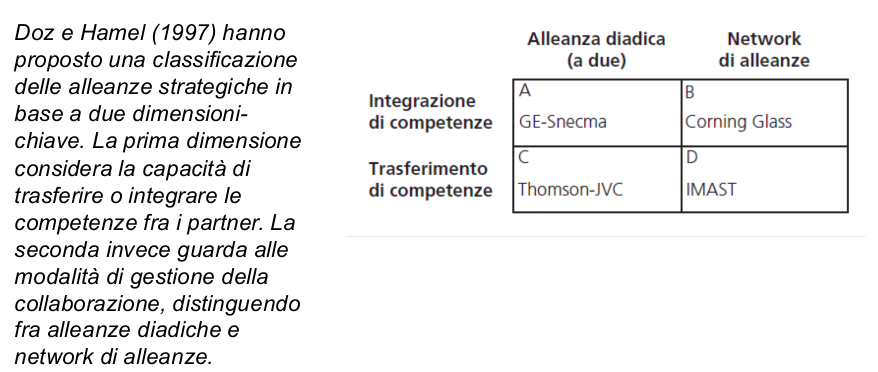
\includegraphics[scale=0.4]{images/allez_stra.png}
	\caption{Alleanza Strategica}
	\label{fig:Porter2}
\end{figure}
\begin{itemize}
\item Integrazione di competenze $\rightarrow$ l’azienda trasferisce ad una o più aziende un componente che
viene integrato nel prodotto da loro realizzato (es. Rolls-Royce produce motori per la Boeing che li
integra nel suo prodotto). Se il trasferimento riguarda due sole aziende si parla di alleanza diadica.
\item Trasferimento competenze $\rightarrow$ l’azienda trasferisce non soltanto il componente ma anche il know-
how che sta dietro la sua realizzazione (passaggio più complesso). Esso può riguardare due sole
imprese o un network di alleanze (es. Ducati che integra dai vari fornitori esterni).
La distinzione non è sempre così netta. 
\end{itemize}


\begin{enumerate}
\item  \textbf{Alleanze strategiche}: accordi di natura formale o informale fra
due o più partner allo scopo di collaborare per una finalità.
\item \textbf{Joint venture}: è una forma particolare di alleanza che richiede ai
partecipanti di adottare una struttura formale, quasi sempre una
nuova entità giuridicamente separata dotata di capitale proprio.
\item \textbf{Licensing}:è un accordo contrattuale che conferisce a
un’organizzazione (o a un individuo) i diritti d’uso di una proprietà
intellettuale di un’altra organizzazione, di norma in cambio di una
royalty.
\item \textbf{Outsourcing}:è una formula in base alla quale un’impresa
trasferisce all’esterno determinati processi piuttosto di realizzarli
al proprio interno.
\item \textbf{Organizzazioni di ricerca}: sono organizzazioni costituite per
favorire la collaborazione fra un gruppo di soggetti, per esempio
imprese ed enti pubblici di ricerca.
\end{enumerate}

\subsection{Alleanze e licensing per stabilire uno standard}
\begin{figure}[h!]
	\centering
	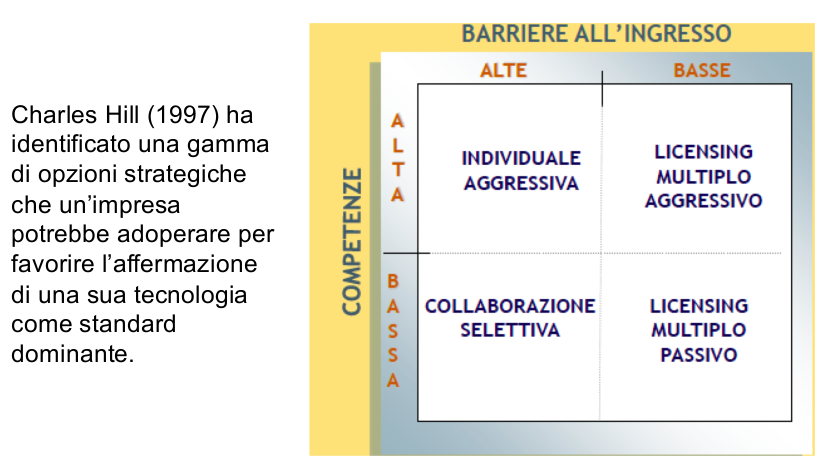
\includegraphics[scale=0.4]{images/licensing.png}
	\caption{Alleanza Strategica}
	\label{fig:Porter2}
\end{figure}

\begin{enumerate}
	\item Individuale – Aggressiva (evita collaborazioni; strategie di diffusione e politiche aggressive
	di prezzo)
	Se si genera un’innovazione e si vuole far affermare questa come dominant design, laddove
	ci siano competenze molto complesse ed alte barriere all’entrata è preferibile una strategia
	individuale. Essendo l’unico produttore c’è maggiore possibilità di affermazione di un
	dominant design poiché ci saranno pochi concorrenti nel futuro. Ciò conviene quando ci
	sono beni complementari e assenza di concorrenti competitivi.
	\item Collaborazione selettiva (alte barriere, basse competenze)
	Si stabilisce un’alleanza per promuovere uno standard, alleanza poiché c’è il rischio che un
	concorrente possa sviluppare la medesima tecnologia o una concorrente. Ciò conviene
	quando il partner è un potenziale concorrente (bassa competenza facilmente acquisibile
	dai concorrenti). L’impresa necessita di risorse in possesso dei concorrenti.
	\item Licensing multiplo aggressivo (tecnologia/conoscenza concessa in licenza)
	Viene trasferita la licenza di una conoscenza a molte imprese (non si sviluppa la conoscenza
	con altre aziende). Persegue strategie aggressive di posizionamento. Conviene in presenza
	di molti potenziali concorrenti (proprie per le basse barriere all’entrata) che potranno
	sviluppare tecnologie diverse.
	\item Licensing multiplo passivo (es. Microsoft, concede il sistema operativo in licenza a tutti i
	produttori di hardware)
	Viene concessa la licenza a tutti gli operatori interessati. Conviene quando ci sono molti
	concorrenti.
\end{enumerate}

\subsection{Scelta e controllo dei partner}
La collaborazione non è una strategia priva di rischi per cui la scelta dei partner giusti è
fondamentale. È difficile stabilire se le risorse fornite dai partner siano adeguate alla propria
impresa. Può anche accadere che qualcuno dei partner sfrutti il rapporto di collaborazione per
appropriarsi di conoscenze senza offrire nulla in cambio. Inoltre, poiché il management può
governare e mantenere sotto il controllo in modo efficace solo un numero limitato di
collaborazioni, l’efficacia di gestione diminuisce all’aumentare del numero di collaborazioni nelle
quali l’impresa è coinvolta.
Scaricato da Giulio Pilotto (pilotto.giulio@gmail.com)lOMoARcPSD|3519035
Il successo di una strategia di collaborazione dipende dai partner che sono stati scelti.
La compatibilità fra i partner può essere influenzata da diversi fattori. Questi fattori possono
essere ricondotti a due dimensioni:
La compatibilità delle risorse: fa riferimento alla potenziale disponibilità nei partner di
risorse che si prestano ad essere integrate e combinate in modo efficace nell’ambito di una
strategia per la creazione di valore. Le risorse dei partner possono essere complementari o
supplementari.
Compatibilità strategica, fa riferimento al grado di allineamento degli obiettivi e degli stili
imprenditoriali dei partner. Tali obiettivi non devono necessariamente coincidere, purché
possano essere perseguiti e raggiunti senza recare danno all’alleanza o agli altri partner.
Gli accordi di collaborazione di maggior successo mostrano meccanismi di governance e di
monitoraggio dei partner ben definiti. In molti casi le parti stipulano accordi contrattuali con
norme vincolanti allo scopo di assicurarsi che ciascun partner sia pienamente consapevole dei
propri diritti e doveri e possa ricorrere alle vie legali in caso di violazione dell’accordo. Nei contratti
si definiscono i seguenti punti:
Il contributo che ciascun partner si obbliga a fornire e a mettere a disposizione della
collaborazione in termini di risorse finanziarie, servizi, ecc.
Il grado di controllo di ciascun partner.
I tempi e i modi della distribuzione di quanto viene generato nel rapporto di collaborazione.
\section{Meccanismo di protezione dell'innovazione}
Nel formulare una strategia di innovazione, un elemento fondamentale è rappresentato dalla
definizione dei meccanismo di protezione delle innovazioni tecnologiche.
A volte, però, è nell’interesse dell’impresa non proteggere l’innovazione, perché incoraggiare altri
operatori (produttori e fornitori di beni complementari) a sostenere la nuova tecnologia può
determinare un più alto tasso di adozione e un processo rapido di diffusione, aumentando la
probabilità di acquisire la posizione di standard dominante.
\textbf{appropiabilità} (concetto opposto a quello di IMITABILITA’)  si intende la capacità
dell’impresa di acquisire e trattenere per sé le rendite generate dai propri processi innovativi. Il
grado di appropriabilità di un’innovazione è determinato dalla facilità e dalla rapidità con cui i
concorrenti riescono ad imitarla (tanto più aumento l’imitabilità tanto minore è la capacità di
appropriabilità). Il grado di imitabilità, a sua volta, è funzione sia della natura delle tecnologia
sviluppata sia dell’efficacia dei meccanismi di protezione adottate.
Se la base di conoscenze è tacita (difficilmente codificabile in documenti o formule) o socialmente
complessa è alquanto improbabile che i concorrenti riusciranno a imitarla o a riprodurla.
Tanto più l’innovazione si basa su conoscenze tacite tanto più l’appropriabilità è alta e l’imitabilità
è bassa.

Brevetti, marchi e copyright costituiscono tutti metodi di protezione della proprietà intellettuale
ma ciascuno è predisposto per la tutela di innovazioni differenti.
Un brevetto protegge un’invenzione; un marchio protegge parole o simboli distintivi della fonte di
provenienza e della proprietà di un bene; il copyright protegge il diritto dell’autore.

\subsection{Brevetti}

Sono delle nuove invenzioni che implicano un’attività inventiva e sono atte ad avere
un’applicazione industriale (valore economico). Il brevetto è una nuova conoscenza che viene
comunicata al fine di essere tutela dal punto di vista giuridico. Tutti i proventi derivanti da essa
sono da attribuire al titolare del brevetto. In mancanza di comunicazione non si può agire contro il
terzo che lo utilizza.
Cosa può essere brevettato?
\begin{itemize}
	\item Novità
	\item Un’innovazione che implichi un’attività inventiva, cioè non sia qualcosa di ovvio, ma
	originale (non possono essere brevettate le scoperte della natura)
	\item Tutto ciò che può avere un’applicazione industriale (che permette un ritorno economico);
	Sia sufficientemente descritta.
	\item Alla base del brevetto c’è la comunicazione della nuova conoscenza (più dettagli più tutela), spesso
	la descrizione del know-how non è abbastanza completa, ciò è causa di numerose battaglie di
	brevetto.
	\item Non possono essere brevettate le scoperte e le invenzioni contrarie all’ordine pubblico.
\end{itemize}

\subsubsection{Strategie Brevettuali}
Uno studio empirico ha messo in evidenza che la maggior parte degli inventori che brevettano preferisce descriverne il contenuto prima ancora che il brevetto venga concesso (disclosure anticipata).Questa scelta permette loro di publicizzare le caratteristiche e l’ambito di applicazione della loro invenzione.La disclosure attraverso la domanda di brevetto stabilisce la data da cui i depositanti possono godere dei primi, provvisori, redditi generati dai diritti di proprietà.
\begin{itemize}
\item Strategie agressive: patent trolling: attraverso una società, patenttroll,che detiene brevetti, una società può minacciare cause legali per strappare lucrose transazioni e ricattare altre imprese. 
\item Patentthicket: fitta ragnatela di brevetti incrociati e sovrapposti per competere senza cadere preda in una  causa in materia dib revetti intentata da imprese concorrenti
\end{itemize}

\subsection{Marchi}
Un \textbf{marchio commerciale} (o trademark) è costituito da una parola, una frase, un simbolo, un
disegno o qualsiasi elemento distintivo della provenienza di un bene. I marchi non riguardano il
know-how o la conoscenza dell’innovazione ma, soltanto il prodotto.
Un marchio di \textbf{servizio} (o service mark) è un marchio
che contraddistingue un fornitore di un servizio

\subsection{Copyright}
Il copyright è una forma di protezione applicabile alle opere soggette a diritto d’autore.L’autore ha il diritto esclusivo di utilizzare economicamente l’opera in ogni forma e modo (nei limiti fissati dalla legge), può rivendicarne la paternità e opporsi a qualsiasi uso che possa pregiudicare la sua reputazioneLa Convenzione di Berna stabilisce un livello minimo di protezione con copyright per tutti i Paesi che hanno aderito.

\subsection{Segreto Industriale }
Il segreto industriale è rappresentato da informazioni di proprietà
esclusiva di un’impresa, che restano ignote all’esterno dell’organizzazione
aziendale.
I segreti industriali non devono rispondere a tutti i rigorosi requisiti previsti
dalle leggi sui brevetti, consentendo la protezione di una più ampia classe
di attività.
L'inforamzione viene ocsnidreata segreto idnustriale se:
\begin{itemize}
	\item Genear unvantagigo distintivo per l'impresa in termini di rnedtia economica.
	\item Conserva il proprio valore rimanendo strettaetmne confidenziale
\end{itemize}

\subsection{Vantaggi della protezione}
\begin{itemize}
	\item   I sistemi proprietari consentono alle imprese di appropriarsi di maggiori rendite (solo
	l’impresa gode dell’appropriabilità).
	\item I profitti generati dall’innovazione possono essere reinvestiti nel miglioramento
	tecnologico.
	\item L’impresa potrebbe essere disposta a subire delle perdite di breve termine perché
	l’affermazione come disegno dominante garantirebbe flussi costanti e duraturi.
	o L’impresa può mantenere il controllo architetturale della tecnologia.
	\item I meccanismi di protezione dell’innovazione e la loro efficacia variano notevolmente a seconda del:
	\begin{itemize}
		\item Settore
		\item Tipologia di innovazione (prodotto, processo, ecc.)(si brevettano maggiormente le
		innovazioni di prodotto)
		\item  Contesto locale (differenze tra Nord e Sud Italia)
	\end{itemize}
\end{itemize}

\subsection{Sistemi Aperti Sistemi Chiusi}
I sistemi aperti permettono a tutti di poter utilizzare la conoscenza.
(caso Arduino, open-source community)
I sistemi proprietari (wholly proprietari system) sono basati sul possesso esclusivo della tecnologia
da parte dell’impresa e su una strategia di protezione.
Talvolta, è nell’interesse dell’imprese non proteggere l’innovazione, perché ciò può determinare
un più alto e un più rapido tasso di adozione e aumentarne la possibilità di divenire lo standard
dominante.
Nei sistemi aperti la tecnologia adottata non è protetta legalmente ed è liberamente accessibile ad
altri produttori.

Vantaggi
\begin{itemize}
	\item Una tecnologia aperta consente e favorisce un processo più rapido di diffusione e adozione
	della tecnologia.
	\item La diffusione della tecnologia senza barriere può favorire la disponibilità di beni
	complementari.
	\item Una tecnologia aperta può beneficiare degli sforzi di sviluppo operati in altre imprese.
\end{itemize}




Fattori che incentivano la scelta tra un sistema aperto o chiuso:
\begin{enumerate}
\item  Capacità di produzione, competenze di marketing e risorse di capitale.
\item  L’opposizione del settore alla tecnologia sole source (a livello di industria era lontana l’idea
di fare open - source, mentre era più facile sul software).
\item Il grado di controllo sui rischi di frammentazione (se la community ha il vantaggio di
migliorare e diffondere il prodotto, ha lo svantaggio di creare tanti prodotti diversi).
\end{enumerate}


In realtà la maggior parte delle tecnologie è riconducibile a situazioni intermedie tra i due sistemi.
Dietro il licensing c’è sempre un brevetto (in genere il brevetto ottimizza i profitti).
ECCEZIONE: nel caso in cui la domanda di mercato di un prodotto è troppo elevata rispetto alla
capacità produttiva dell’azienda, può convenire il licensing (la parte del mercato aggiuntiva è
coperta dai guadagni derivanti dal licensing).

\section{Organizzazione dei processi di innovazione}
Il ruolo dell'Organizzazione nella performance aziendale
\begin{itemize}
\item Strutture organizzative che incoraggiano la creatività e l’innovazione
\item Strutture che garantiscono una maggiore efficienza dei processi di
produzione di nuovi prodotti
\item Strutture che permettono di soddisfare entrambi gli obiettivi appena
elencati (scambio interno del personale, sistemi di controllo, strutture
imprenditoriali)
\end{itemize}

La gestione e il coordinamento delle attività di sviluppo
dell’innovazione sono particolarmente complesse

L’impresa accumula conoscenza all’interno della sua organizzazione
(routine per risolvere problemi, guidare azioni,...) e il suo obiettivo è
quello di preservare la conoscenza ottenuta.
Come?
Apprendimento e ricerca...per risolvere problemi
Organizational learning is the growing insights and succeful
restructuring of organizational problems by individuals reflected in
the structural elements and outcomes of the organization itself
(Simon, 1969)

\subsection{Organizzazione e dimensione di impresa}
Schumpeter (1942) sosteneva che la \textbf{capacità d’innovazione} delle
grandi imprese è superiore a quella delle piccole imprese, perché
\begin{itemize}
	\item Il mercato dei capitali è imperfetto
	accesso più facile ai capitali
	\item Hanno maggiori volumi di vendita sui quali ripartire i costi di R\&S
	\item  Possesso di beni complementari più evoluti (es. pianificazione
	finanziaria)
	Altri vantaggi legati alla grande dimensione:
	\item  Maggiori economie di scala e di apprendimento (acquisizione di
	nuove competenze)
	\item  Assunzione di progetti rischiosi o di grandi proporzioni
\end{itemize}

La grande dimensione può svantaggiare l’innovazione:

\begin{itemize}
\item	 minore efficienza della R\&S a causa di una perdita di controllo manageriale
\item maggiore inerzia burocratica contro i cambiamenti rapidi (paradosso
di Icaro)
\item più elevato grado di commitment strategico che tende a vincolare
l’impresa alle tecnologie esistenti
\item Le piccole imprese sono spesso considerate più flessibili e con un
maggior spirito imprenditoriale. Selezionano con maggior cautela i
progetti innovativi (tasso di successo più elevato nell’innovazione di
prodotto)
\end{itemize}


\textbf{Xerox  Il paradosso di Icaro}
i campi di eccellenza possono rivelarsi la causa della rovina

Se le dimensioni aziendali rappresentano un vincolo come
introdurre i sistemi e la mentalità della piccola impresa?

\begin{itemize}
\item 	attraverso la scomposizione e distribuzione delle attività in
	unità più piccole (diffondere una mentalità imprenditoriale,
	maggiore livello di specializzazione)
\item culture e meccanismi di controllo differenti nelle diverse unità
	(nuove formule organizzative)

\end{itemize}

\subsection{Le variabili strutturali della dimensione d'impresa}

\begin{itemize}
\item	Per formalizzazione si intende il grado di regolazione del
	comportamento dei membri di un’organizzazione attraverso regole,
	procedure e documentazioni prodotte in forma ufficiale.
	La formalizzazione permette di attenuare l’intensità dei meccanismi di
	controllo organizzativo e mantenere l’efficienza gestionale.
	Attenzione!: procedure prestabilite possono soffocare la creatività del
	personale
	\item Per standardizzazione si intende il grado di codificazione delle attività
	dell’impresa secondo procedure, regole e comportamenti
	predeterminati. Ha lo scopo di regolare lo svolgimento di tutte le attività
	per il conseguimento dei risultati attesi.
	La standardizzazione rischia di limitare la creatività
	
	\item Per accentramento si intende:
	 il grado di concentrazione del potere decisionale al vertice dell’impresa
	oppure.
	il grado di concentrazione geografica delle attività principali.
	Al contrario, il decentramento prevede la distribuzione del potere
	all’interno di tutta la struttura organizzativa
	
	\item Per le imprese che si dedicano a più progetti di innovazione in
	contemporanea la scelta di accentrare o decentrare le attività di R\&S è
	l’esito di un processo decisionale complesso.
	Il settore influisce sulla scelta:
	Beni di consumo: decentramento di R\&S
	Elettronica: concentrazione di R\&S
\end{itemize}

\subsection{Strutture meccaniche e organiche}
La combinazione di formalizzazione e standardizzazione configura una
\textbf{struttura meccanica} capace di garantire alti livelli di efficienza per livelli
di produzione elevati.
L’adozione di comportamenti basati sul rispetto delle regole di
condotta e delle procedure aziendali assieme ad un alto livello di
standardizzazione delle attività aziendali rende un’impresa una
macchina efficiente (Adler, 1999).
Tuttavia, le strutture meccaniche sono giudicate incompatibili o
inadatte ad una strategia che incoraggi l’innovazione.
La loro efficacia si basa sul rispetto degli standard e la riduzione
di varietà e variabilità dei comportamenti....ciò genera un
soffocamento della creatività.
Le strutture organiche concedono maggiore libertà di decisione e sono
caratterizzate da bassi livelli di formalizzazione e dall’assenza di
standardizzazione. Sono più adatte per attività creative e innovative e per
contesti competitivi dinamici
\begin{itemize}
	\item Viene concessa maggiore autonomia
	\item Ampia discrezionalità nelle procedure organizzative e schemi
	d’azione da seguire
	\item  Viene favorita la sperimentazione e l’improvvisazione

\end{itemize}
Struttura coerente con i processi di innovazione, tuttavia possono portare
a riduzioni di efficienza dell’impresa.

Molti dei vantaggi e dei limiti delle dimensioni organizzative sono
collegati a variabili strutturali, come il grado di formalizzazione, di
standardizzazione e di accentramento
Le grandi imprese tendono a ricorrere
maggiormente alla formalizzazione e alla
standardizzazione, in quanto con la crescita
dimensionale diviene più difficile esercitare un
controllo manageriale diretto


\subsection{Organizazzione Ambidestra}
L’organizzazione ambidestra (o ibrida) è una forma complessa
costituita da una molteplicità di “architetture interne”
ü In alcuni contesti o aree aziendali (per esempio, la produzione) il
management potrebbe adottare strutture meccaniche; in altri (per
esempio, la R\&S), strutture organiche.
\begin{itemize}
\item In ciascuna area o unità, l’organizzazione potrebbe essere
ridisegnata per focalizzarsi su obiettivi particolari (skunk work,
task force, team di progetto).
\item Per combinare i vantaggi delle strutture meccaniche e organiche, i
due modelli possono essere anche alternati nel tempo.
\end{itemize}

\subsection{Modularità dei prodotti}
Altro metodo per trovare un equilibrio tra efficienza e flessibilità
consiste nell’adottare componenti standard o di piattaforme di
produzione e tecnologiche condivisibili.
la modularità, cioè la scomponibilità e ricombinazione dei componenti
di un sistema, consente un più ampio ventaglio di configurazioni
finali partendo da un insieme di componenti base.
Rappresenta pertanto una soluzione economicamente vantaggiosa per
rispondere all’eterogeneità della domanda di mercato.
\begin{itemize}
\item  Maggiore la modularità dei prodotti,
\item  Minore il rischio di restare intrappolati in una singola configurazione
\item Maggiore la probabilità di cogliere le opportunità di mercato.
La modularità dei prodotti rende l’intero sistema di produzione modulare!
\end{itemize}


\subsection{Strutture Loosely Coupled}
Nelle strutture loosely coupled le attività non
sono strettamente integrate e il coordinamento
fra due processi avviene attraverso l’adesione
a obiettivi condivisi e standard comuni

Le tecnologie dell’informazione riducono il bisogno di integrazione e il
minore bisogno di integrazione consente alle imprese di ricercare
configurazioni più flessibili
Per esempio, un’impresa può concentrare
l’impegno sulle attività correlate alle proprie
competenze distintive e affidare in outsourcing
le altre
Tali strutture non sono adatte per attività che richiedono frequenti scambi
di conoscenza

\subsection{La gestione dei processi interazionali di innovazione}
La scelta delle modalità di organizzazione è
un’area particolarmente critica per le imprese
internazionali
In particolare assume un ruolo decisivo
l’identificazione della combinazione ideale tra
integrazione globale e adattamento ai mercati
locali
L’innovazione sviluppata per un particolare mercato
potrebbe non essere efficacemente trasferita nei
altri mercati (sindrome del non inventato qui)

Bartlett e Ghoshal hanno identificato quattro tipi di strategie di innovazione
delle imprese internazionali.

\begin{itemize}
\item  Cenetr-for-global-innoavation:le attività di R\&S sono
concentrate in un’unica sede
principale e il processo di
innovazione si identifica con
un trasferimento e un
adattamento di tecnologia dal
centro alle unità locali.
Il management mantiene il
controllo sul processo di
sviluppo dell’innovazione

\item Local-for-local innovation
ogni sede nazionale sviluppa un
processo di innovazione
destinato a rispondere alla
domanda del mercato locale
Viene privilegiata l’identità e
l’autonomia delle consociate

\item Local-for-global innovation
Attività di R\&S che fanno parte
di una rete globale. I risultati
sono trasferiti all’intera
organizzazione

\item Global-for-global innovation
Attività di R\&S che fanno parte
di una rete globale. I risultati
sono trasferiti all’intera
organizzazione Collaborazione con altre unità di
R\&S localizzate in diversi luoghi
geografici.
Combinazione del pool di
competenze e di risorse per una
condivisione internazionale.
\end{itemize}

\section{Gestione dei Team per lo sviluppo di un prodotto}
\subsection{Il caso Disney}
Walt Disney Company, fondata nel 1923 come casa produttrice di film di animazione, è
ormai un conglomerato dell’industria dell’entertainment, con oltre 50 miliardi di dollari di
ricavi e 185mila dipendenti.
Per lungo tempo, il processo di sviluppo di un nuovo film animato veniva gestito inizialmente
da un incubation team per il concept e in seguito da 5 team autonomi focalizzati su diversi
aspetti informatici (data center, rendering, backup, supporto tecnico) fino alla post-
produzione.
Geibel, direttore della divisione Sistemi, aveva osservato che il contributo individuale
(qualità del confronto e della discussione) a un progetto tendeva a calare all’aumentare del
numero dei membri del team.
Decise così di ridimensionare i team e di designare nuovi team leader in base alle
competenze manageriali e non alla seniority. Ciascun team avrebbe operato in piena
autonomia come una start-up assumendo la responsabilità dell’intero processo per l’area di
competenza assegnata, con un orientamento al risultato.
Geibel, inoltre, intervenne sulla struttura dello spazio di lavoro. Stabilì che i team dovessero
condividere lo stesso spazio fisico, per favorire le relazioni personali e lo scambio di
informazioni: la prossimità è la chiave.
All’inizio il processo di creazione di una "cultura creativa" ha incontrato non poche
resistenze, soprattutto fra tecnici e ingegneri non abituati ad operare in autonomia:" ci vorrà
del tempo per adattarsi a una nuova cultura dove ci si attende che ciascuno sfidi lo status
quo e che il pensiero critico sia presente a tutti i livelli".

Che cosa influisce sulla performance di un team di sviluppo di
nuovi prodotti?
\begin{itemize}
\item La dimensione
\item La composizione
\item La struttura
\item La gestione
\item Gli stili di leadership
\end{itemize}

\subsection{Dimensione}
\begin{enumerate}
\item La dimensione dei team di sviluppo varia a seconda delle imprese
(GI, PMI)
\item  Le dimensioni possono variare durante la vita del progetto
\item  La grande dimensione non costituisce sempre un vantaggio,
perché può comportare un aumento dei costi di gestione e
amplificare i problemi di comunicazione
\item Con l’aumento delle dimensioni tendono ad aumentare i rischi di
inerzia sociale (fenomeno legato ad un riconoscimento sociale
non adeguato allo sforzo del singolo all’interno del gruppo)
\end{enumerate}

La collaborazione di esperti con background differenti
estende la base di conoscenze all’interno del gruppo,
favorendo la cross-fertilization e lo scambio di idee.
Anche altri tipi di eterogeneità nei team (diversità culturali, di età, di
sesso ecc.) possono favorire i processi di innovazione.
I gruppi eterogenei dovrebbero avere a disposizione una più ampia base di
conoscenze (varietà e quantità) rispetto ai gruppi omogenei.
Eterogeneità del team, varietà delle relazioni e apertura a fonti esterne sono
fondamentali nel determinare i processi di innovazione delle imprese creative
Le diversità interne ai team possono comportare maggiori costi di
coordinamento e difficoltà di comunicazione
Le scienze dell’organizzazione evidenziano che le differenze fra i
team “omogenei” ed “eterogenei” negli aspetti di comunicazione e di
coordinamento si attenuano se il contatto all’interno del gruppo si
protrae nel tempo.
Ancona e Caldwell (1997) hanno condotto uno studio su 45 team
individuando le principali attività svolte lungo i confini fra
organizzazione e ambiente (boundary-spanning):
\begin{enumerate}
	\item ambasciatori: attività dirette a rappresentare il team verso
	interlocutori esterni;
	\item coordinamento di compiti: attività di coordinamento e
	negoziazione del team con altri gruppi;
	\item  scouting: attività finalizzate a esplorare idee e informazioni utili
	per il team.
\end{enumerate}

Le attività di scouting e di “ambasciatori” comportavano molti benefici
se svolte nelle prime fasi del processo di sviluppo; quelle di
coordinamento dei compiti, invece, durante tutta la vita del progetto.

Kichuk e Wieser (1997) hanno evidenziato che cinque fattori della
personalità infuiscono sulle probabilità di successo del team:
\begin{itemize}
\item Senso di responsabilità
\item Estroversione
\item Irritabilità
\item Disponibilità
\item Apertura a nuove esperienze
\end{itemize}


\subsection{Alleanze e licensing per stabilire uno standard}
\begin{figure}[h!]
	\centering
	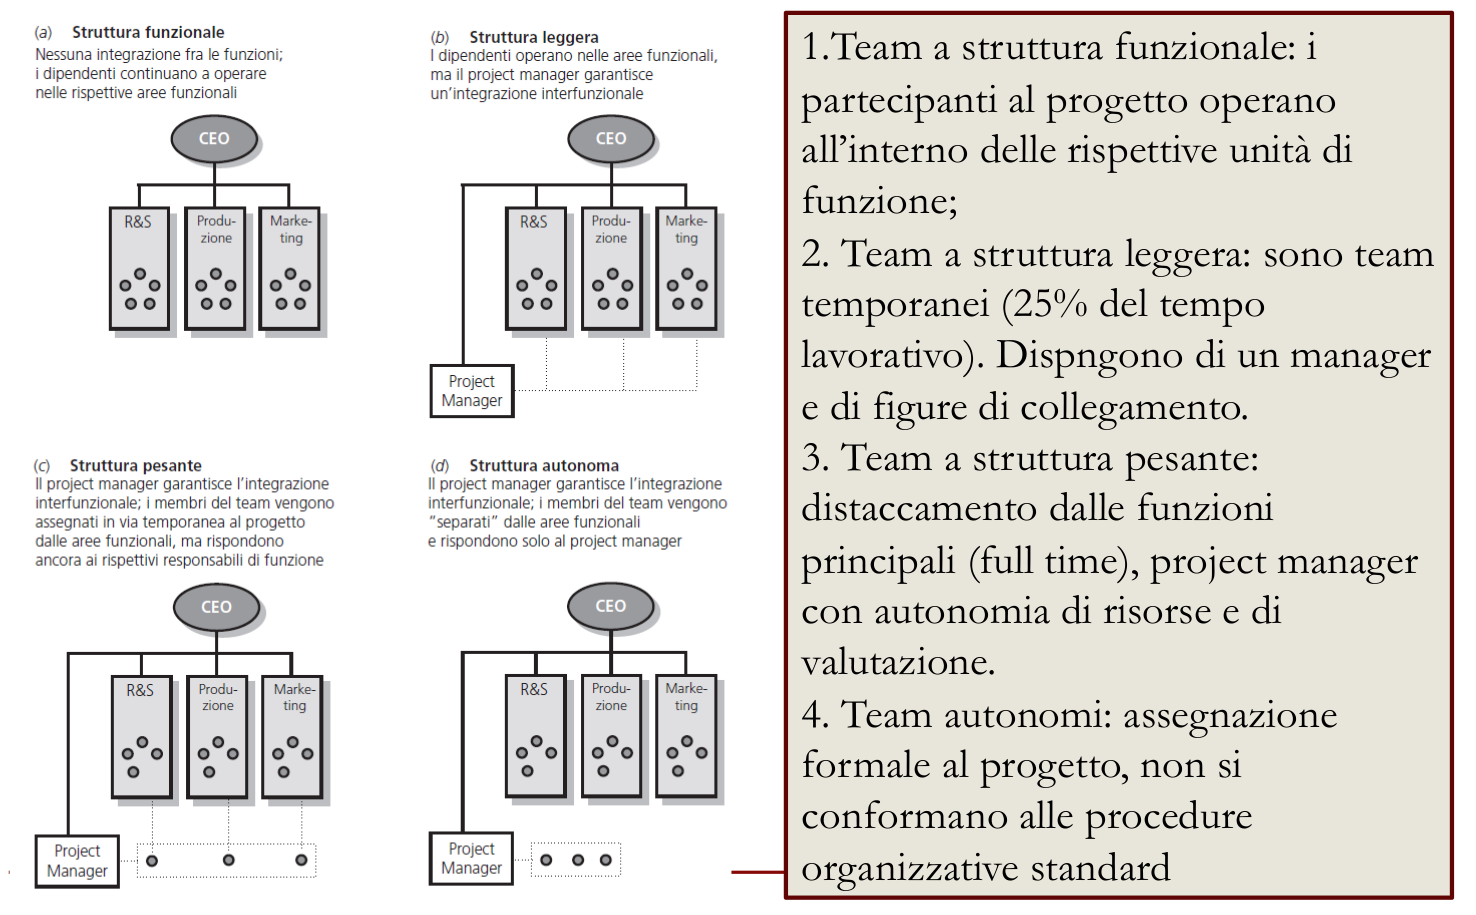
\includegraphics[scale=0.4]{images/ceo.png}
	\caption{Struttura dei team di sviluppo di nuovi prodotti}
	\label{fig:team}
\end{figure}

\subsection{Leadership del team }
Il team leader ha la responsabilità di:
\begin{itemize}
\item guidare le attività del team
\item mantenere l’allineamento del gruppo agli obiettivi del
progetto
\item comunicare con il vertice aziendale
\end{itemize}

Per ogni tipologia di team esiste una diversa figura di leader.
Ad es., i team leggeri possono essere guidati da un manager di
livello intermedio che si limita al coordinamento di base mentre un
team pesante o autonomo ha bisogno di un manager di grande
esperienza con una dose di autorità all’interno dell’organizzazione.

Il \textbf{project charter} racchiude la missione del progetto e descrive con
una definizione precisa gli obiettivi da raggiungere, indicandone i
criteri di misurazione. Può anche precisare:
\begin{itemize}

\item i componenti del team
\item la durata prevista della partecipazione al progetto
\item la percentuale di ore da dedicare alle attività del team
\item il budget
\item le scadenze intermedie
\item  gli indicatori di successo del progetto

\end{itemize}


Nei \textbf{team virtuali}:
\begin{itemize}
\item  i membri, pur essendo dislocati in aree geografiche anche molto
distanti tra loro, riescono a mantenere un’intensa collaborazione
mediante strumenti di comunicazione avanzati (videoconferenza,
e-mail, programmi di chat).
\item  I membri del team devono essere capaci di svolgere compiti
assegnati in autonomia e possedere una forte etica della
responsabilità.
\item  Sono uno strumento di grande utilità per le imprese che operano
su scala globale
\item  Limiti: ostacoli nella creazione di un codice e di un linguaggio
condivisi
\end{itemize}

\begin{figure}[h!]
	\centering
	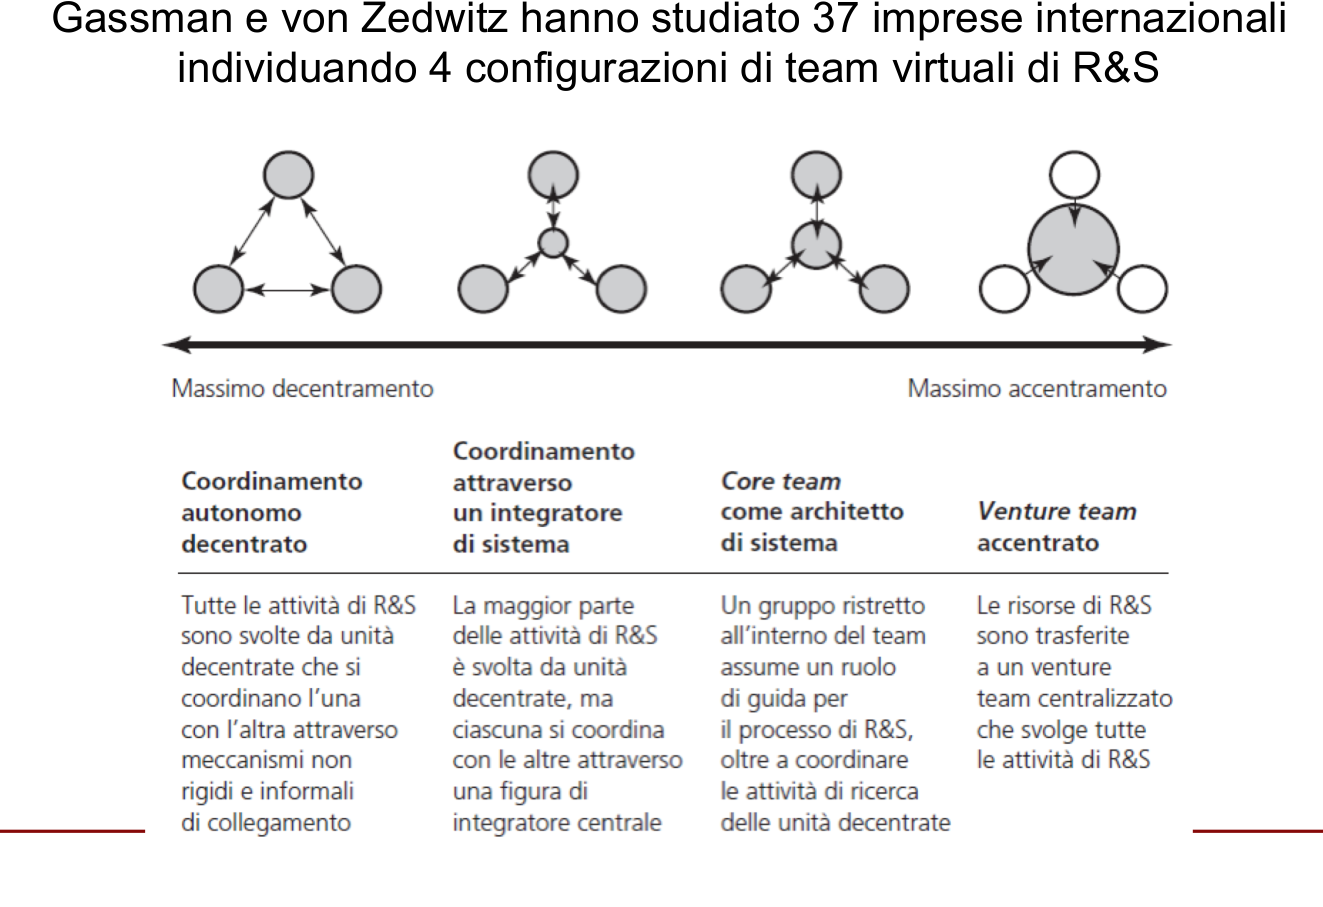
\includegraphics[scale=0.4]{images/virtuali.png}
	\caption{Struttura dei team di sviluppo di nuovi prodotti}
	\label{fig:virtuali}
\end{figure}

efficacia ed efficienza
nell’esecuzione
Ciascuno stadio di
sviluppo presenta in
genere costi superiori
alla fase precedente; la
scomposizione in tappe
ripartisce l’investimento
in impegni progressivi;
la spesa complessiva
aumenta solo quando si
riduce il grado di
incertezza

\subsection{Quality funcition Deployment}

Per costruire la matrice del QDF occorre:
\begin{enumerate}
	\item identificare le preferenze e le esigenze del cliente
	\item valutare le preferenze e le esigenze del cliente
	\item individuare le caratteristiche tecniche di progettazione che
	determinano la performance del prodotto
	\item inserire nella matrice il grado di correlazione fra le
	caratteristiche tecniche del prodotto
	\item compilare il corpo centrale della matrice
	\item	moltiplicare i valori che rappresentano l’importanza
	percepita dal cliente per ciascun attributo per il grado di
	relazione tra le due variabili determinato nella fase
	precedente
	\item	confrontare le differenti offerte della concorrenza
	\item	stabilire i valori target per ciascun elemento progettuale
	\item	valutare il nuovo design progettato alla luce dei target stabiliti
\end{enumerate}
\section{Lo sviluppo di un nuovo prodotto}

Come si può aumentare l’efficienza e l’efficacia del processo di
sviluppo di nuovi prodotti?
Impariamo alcune indicazioni strategiche: 3 obiettivi principali
\begin{itemize}
	\item Come rendere massima la capacità di risposta alle richieste e
	alle esigenze del cliente;
	\item  Come ridurre la durata del ciclo di sviluppo
	\item  Come mantenere sotto controllo i costi del processo
\end{itemize}

\subsection{Massimizzare la soddisfazione del cliente}
Il nuovo prodotto deve creare valore per il cliente (maggiore qualità
o prezzo più conveniente)
Molti progetti di sviluppo non riescono a soddisfare questi requisiti.
Perché?
\begin{itemize}
	\item Idea confusa o distorta degli attributi del prodotto
	\item  Le imprese sopravvalutano la disponibilità del cliente a spendere
	\item  L’impresa non riesce a soddisfare una domanda molto
	eterogenea
	\item  Aspetti tecnologici dei prodotti troppo sofisticati
\end{itemize}

\subsection{Ridurre il cliclo di vita dello sviluppo }
I prodotti rischiano di fallire se arrivano al mercato troppo tardi.
Una durata breve di sviluppo del prodotto significa:
\begin{itemize}
	\item A parità di condizioni, i prodotti che entrano per primi nel mercato
	tendono ad acquisire un maggior vantaggio in termini di base di clienti
	e di installazioni e disponibilità di beni complementari.
	\item Controllo e riduzione dei costi di sviluppo. I costi sono direttamente
	correlati al tempo di sviluppo. Più i tempi sono lunghi più difficile
	l’ammortamento totale dei costi di sviluppo.
	\item  Possibilità di modificare o migliorare la propria offerta grazie alla
	conoscenza dei limiti del prodotto esperiti dai consumatori oppure
	grazie a nuove opportunità offerte dal progresso tecnologico.
\end{itemize}

er molto tempo, la maggior
parte delle imprese ha
adottato processi di
sviluppo sequenziali;
oggi, invece tendono a
prevalere processi
simultanei (o a fasi
parallele)
I processi paralleli
abbreviano i tempi di
sviluppo e consentono un
maggiore coordinamento tra
le fasi. Tuttavia, in alcuni casi
questa modalità può
comportare un aumento dei
costi.

\subsection{Project Champion }
Alcuni studi hanno suggerito la designazione di un senior manager per
difendere il progetto di sviluppo di un nuovo prodotto (di qui project
champion)

Benefici:
\begin{itemize}
	\item Ha il potere e l’autorità per
	sostenere e difendere il progetto
	\item Può influire sull’allocazione delle
	risorse
	\item Può incoraggiare la
	comunicazione fra le unità
	organizzative
	
\end{itemize}

Rischi:
\begin{itemize}
	\item Può rimanere intrappolato
	nell’escalating commitment
	\item  Può scoraggiare l’opposizione di
	altri membri al progetto anche
	quando è difficile che crei valore
	\item  Può fornire un giudizio offuscato
	sul valore del progetto
\end{itemize}

cinque falsi miti dei project champion
Markham e Aiman-Smith hanno individuato nelle loro ricerche alcuni
falsi miti sui project champion. Secondo i dati raccolti, non è sempre
vero che:
\begin{enumerate}
	\item i progetti che si avvalgono di un champion hanno più
	probabilità di avere successo nel mercato;
	\item il coinvolgimento dei champion è determinato dal desiderio di
	partecipare al progetto, piuttosto che dal proprio interesse
	personale;
	\item la partecipazione di champion avviene con maggiore
	probabilità in progetti di innovazione radicale;
	\item i champion provengono con maggiore probabilità dai vertici
	dell’organizzazione;
	\item i champion provengono con maggiore probabilità dall’area
	del marketing.
\end{enumerate}

\subsection{Coinvolgimento Dei clienti e di efronitori nel processo di sviluppo}
Molti prodotti non generano un ritorno economico perché non soddisfano le esigenze del cliente
in termini di performance o di prezzo, o perché i tempi di sviluppo e di commercializzazione sono
troppo lunghi. L’impresa può tentare di risolvere questi problemi coinvolgendo i clienti e i fornitori
nel processo di sviluppo.

\subsubsection{Coinvolgimento dei clienti}
Coinvolgere il cliente nel team di sviluppo o consentire agli utilizzatori di sperimentare versioni di
prova del prodotto, è una scelta strategica che permette all’impresa di concentrare i propri sforzi
di sviluppo su progetti in grado di soddisfare in misura maggiore le esigenze della domanda di
mercato. allo scopo di ottenere informazioni e suggerimenti da parte dei propri clienti fin dalle
prime fasi del processo di sviluppo dell’innovazione, molte imprese ricorrono al beta testing. Con
esso l’impresa segnala al mercato le caratteristiche base del nuovo prodotto prima della sua
versione definitiva. Altre imprese coinvolgono i clienti nel processo di sviluppo del nuovo prodotto
anche in modi più intensi, come consentendo loro di co – creare il prodotto finale. Talvolta, i lead
user, ovvero gli utilizzatori che sperimentano come pionieri i nuovi prodotti, sono fondamentali
per testare le nuove tecnologie, correggere gli errori di progettazione e perfezionare la soluzione
definitiva.

\subsubsection{Coinvolgimento dei fornitori}
La base di conoscenze dei fornitori rappresenta un’importante fonte di informazioni a cui
l’impresa può attingere; quindi il management può decidere di includere i fornitori nel team di
prodotto o di consultarli in qualità di partner. In entrambi i casi, i fornitori possono contribuire con
nuove idee al miglioramento del prodotto o all’aumento dell’efficienza del processo di sviluppo
(es. il fornitore può suggerire una risorsa o un componente alternativo in grado di offrire la stessa
funzionalità ma a costi più competitivi). Inoltre coordinando i processi operativi della propria
azienda con le attività svolte dai fornitori, il management può minimizzare i tempi di sviluppo:
maggior tempestività nell’accesso alle risorse e agli altri fattori di produzione e maggior rapidità
nell’apportare eventuali modifiche al progetto.
La ricerca empirica ha dimostrato che molte imprese riescono a produrre nuovi prodotti in tempi
più brevi con costi più bassi e standard di qualità più elevati integrando i fornitori all’interno dei
processi di sviluppo.

\subsection{Crowdsourcing}
Il crowdsourcing è un modello basato sulla condivisione di conoscenze
su larga scala per l’ideazione, lo sviluppo e la realizzazione di progetti.
È la pratica di collaborazione di massa a processi complessi di ricerca e di
innovazione, di norma attraverso l’uso di piattaforme digitali.

\subsection{Progetti stage-gate}
Introdurre punti di sbarramento (go/kill decision points) riduce il rischio di
sostenere a lungo progetti il cui valore atteso è divenuto negativo

Prima di ogni stadio il
progetto deve superare
un punto di
sbarramento, allo scopo
di verificarne validità,
efficacia ed efficienza
nell’esecuzione
Ciascuno stadio di
sviluppo presenta in
genere costi superiori
alla fase precedente; la
scomposizione in tappe
ripartisce l’investimento
in impegni progressivi;
la spesa complessiva
aumenta solo quando si
riduce il grado di
incertezza

\subsubsection{Quality funcition Deployment}

Per costruire la matrice del QDF occorre:
\begin{enumerate}
	\item identificare le preferenze e le esigenze del cliente
	\item valutare le preferenze e le esigenze del cliente
	\item individuare le caratteristiche tecniche di progettazione che
	determinano la performance del prodotto
	\item inserire nella matrice il grado di correlazione fra le
	caratteristiche tecniche del prodotto
	\item compilare il corpo centrale della matrice
	\item	moltiplicare i valori che rappresentano l’importanza
	percepita dal cliente per ciascun attributo per il grado di
	relazione tra le due variabili determinato nella fase
	precedente
	\item	confrontare le differenti offerte della concorrenza
	\item	stabilire i valori target per ciascun elemento progettuale
	\item	valutare il nuovo design progettato alla luce dei target stabiliti
\end{enumerate}

\subsubsection{Design fro Manufacturing}
\begin{figure}[h!]
	\centering
	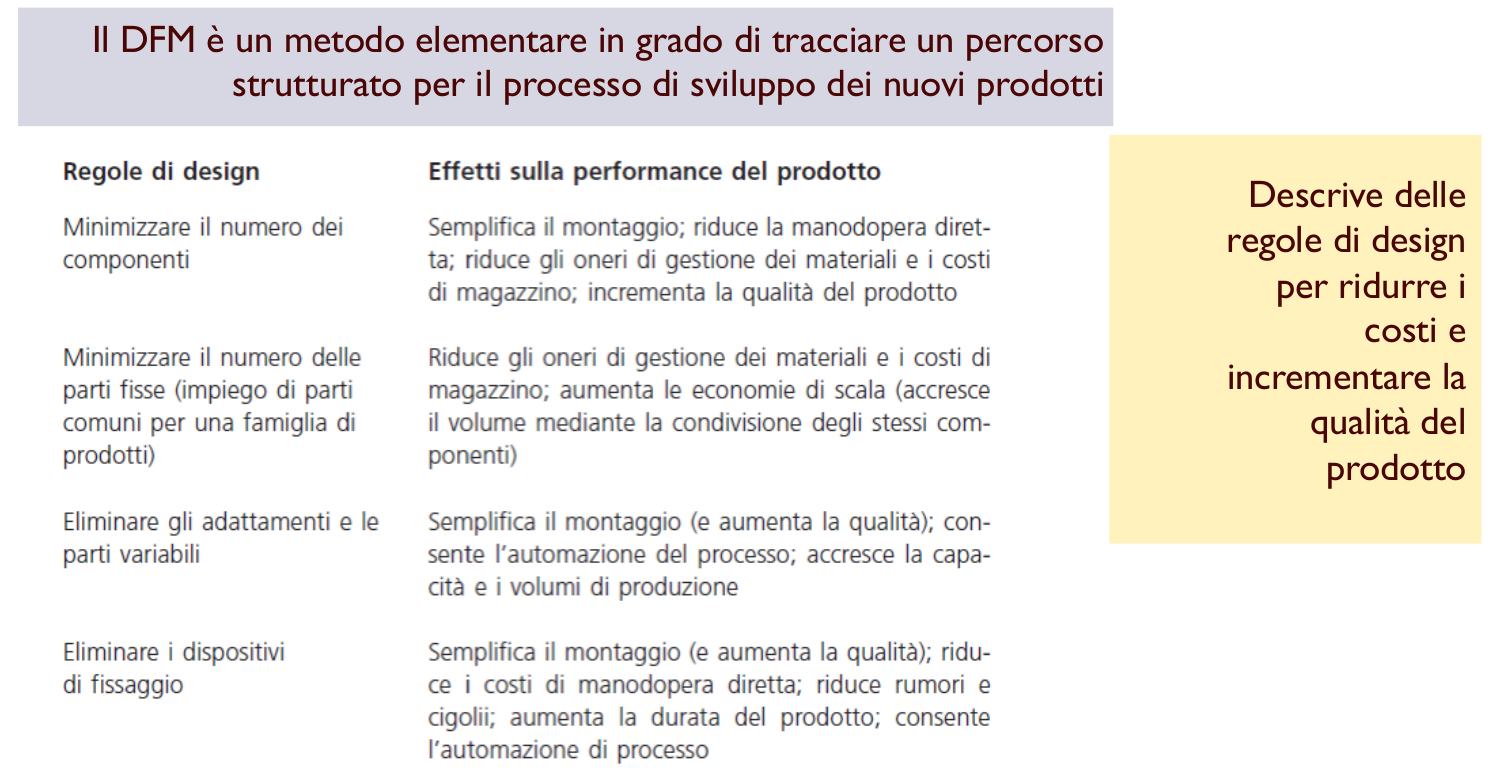
\includegraphics[scale=0.4]{images/DFM.png}
	\caption{Pensiero Capitalista}
	\label{fig:DFN}
\end{figure}

\subsection{Misurazione della performance}
Misurare la performance dei processi di sviluppo di
nuovi prodotti consente al management di migliorare
le strategie e i processi di innovazione

\begin{itemize}
	\item dirata media del ciclo di sviluppo
	\item percentuale di progetti che rispetta le scadenze prefissate
	\item quanti progetti sono rimasti dentro il budget prefissato 
	\item quanti progetti sono diventati un prodotto finito vendibile nel mercato
\end{itemize}

\section{Circular Economy}

\begin{itemize}
	\item \textbf{Linear economy} : Take $\rightarrow$ Make  $\rightarrow$ Distribuite $\rightarrow$ Consume  $\rightarrow$ \textbf{ Dispose}
	\item \textbf{Circular Economy} :  Take  $\rightarrow$ Make  $\rightarrow$ Distribuite $\rightarrow$Consume  $\rightarrow$  \textbf{Return}
\end{itemize}



\begin{itemize}
	\item Undestand $\rightarrow$ How to source what it needs?
	\item Manage  $\rightarrow$ How to create Value?
	\item Develop  $\rightarrow$ What kind of buisiness model?
\end{itemize}

Il problema principale di un economia lineare è che si crea una scarsità di risorse e una quanitità di rifiuti tossici per l'ambiente.

\textbf{Sustainable development}
It is seen as the process of satisfying the current needs of the population without compromising the
capacity to do so of future generations.

\textbf{Sustainability}
It is often understood as the protection of non-renewable natural resources, biodiversity and avoidance
of climatic changes.
With the main focus being on environmental issues this type of sustainability is also framed as ecological
sustainability. There is also social sustainability defined as sustainability that “refers to actively supporting
the preservation and creation of skills as well as the capabilities of future generations, promoting health
and supporting equal and democratic treatments that allow for good quality of life both inside and
outside of the company context.

Sustainability can be seen as part of sustainable development and the latter term describes
the transition process towards a sustainable world.
The circular economy can be understood as a concept contributing to this transition process.

The sustainability revolution: the three pillars
It is based on the often called three E’s:
\begin{itemize}
	\item ecology/ environment,
	\item economy/ employment,
	\item equity/ equality
\end{itemize}

The sustainability revolution requires a transition implying changes in technologies,
infrastructure, lifecycles and institutions as well as in structures of consumption and production
that are radical, long-term and far-reaching.

This means that a system innovation for the sustainability goal is required.
A system innovation can be described as a combination of innovations on various levels to
provide service in a new way.
This entails a socio-technical change with new ways of practice and consumption. The term
socio-technical in this context means that this change does not only affect a technological
change but in addition it requires a modification of social patterns. These fundamental shifts
usually take several decades and require an interplay between a variety of actors such as
policy makers, knowledge-generating institutions, companies and customers.

\subsection{Does sustainability mean to limit the growth?}
The question should not be if economic growth can be combined with environmental concerns but
how growth can be combined with preservation of the environment.
Resource productivity and eco-efficiency play an important role in the context of environmental
concerns and lead to the concept of decoupling.
This concept has the objective of reducing resource depletion and environmental impact while
ensuring economic growth (United Nations Environment Program 2011).
Decoupling can be understood as an important factor to ensure long-term economic growth
under the condition of sustainable development (using less material, energy, water as well as
land resource and reusing material)The UNEP International Resource Panel defines two aspects of the decoupling:
The resource decoupling means reducing the rate of use of resources per unit of
economic activity, and the impact decoupling means maintaining economic output while
reducing the negative environmental impact of the underlying economic activities.

\subsection{Circular Economy }

An economy that provides:
multiple VALUE creation
mechanisms which are decoupled
from the consumption of FINITE
RESOURCES
\begin{itemize}
	\item Design out waste
	\item Build resilience
	through diversity
	renewable sources
	\item  Think systems cascades
	\item The CE thinking requires the application of 3 PRINCIPLES that together
	lead to an economy that is prosperous while being natural capital
	restorative and regenerative
	\begin{itemize}
		\item preserve and enhance natural capital
		\item  optimase resourse yield (Tehnical and Biological cycles)
		\item foster system effectiveness (no - env esternalities)
	\end{itemize}
\end{itemize}

\subsection{Transition Tu circular economy}
Four important blocks:
\begin{itemize}
	\item materials and product design,
	\item new business models,
	\item  global reverse networks, and
	\item enabling conditions :Education ,Financing, Collaborative platform , New economic framework for pricing externalities
\end{itemize}

\subsection{Circular Business Model }
Business Model: the rationale of how an organization creates,
delivers and captures value.

Purpose “profit/value/ well-being”
describes the design/architecture/framework
of the mechanisms employed of value.

\textbf{Circular Business Model}
Strategic systemic thinking to gain Circular advantages
Innovate :Productivity of resources ,
Value within the whole life cycle of the product.

\subsubsection{Example of Circular Business Model}
\begin{enumerate}
\item \textbf{Circular supply chain }
	\begin{itemize}
		\item Circular process : regain Value from components/waste/products at
		the end of their cycle:closed: product from inside the
		company , open: product from other companies
		\item Objective : Gain access to renewable and recycled
		Inputs
		\item advantages
		More independence from external
		resources (decouple production from
		shocks, resource unavailability,
		volatility of price.
	\end{itemize}
	\item  Extension of lifecycel
	\item sharing 
	\item Product as a Service
\end{enumerate}

\subsection{Policies for a circular economy}

\section{Le strategie di distribuzione}
\begin{itemize}
	\item Vendita diretta : Maggiore controllo su
	processo
	di vendita, prezzo e servizio.Può essere troppo costosa o
	poco pratica
	\item Vendita tramite
	intermediari (Rappresentanti, Grossisti): Attività di servizio (maggiore
	efficienza),Servizi correlati
\end{itemize}

Per stabilire se avvalersi di intermediari e quale tipologia di
intermediario è più adatta, il management dovrebbe porsi e
rispondere ad alcune domande.
Il nuovo prodotto presenta le stesse esigenze di
distribuzione delle linee già esistenti?
Quanti sono i clienti? Dove sono situati? Quanta
“formazione” all’uso del prodotto e quanti servizi
dovranno essere forniti? E’ consigliabile o indispensabile
la prova del prodotto prima dell’acquisto? Il prodotto
richiede di essere installato da parte di personale
specializzato o di essere adattato alle esigenze del
cliente?
Come vengono venduti i prodotti concorrenti o sostitutivi?

\begin{itemize}
	\item Pubblicità: Richiede un messaggio efficace,
	Occorre coerenza tra il media utilizzato e il
	target, 
	Occorre trovare un equilibrio fra un
	messaggio semplice da ricordare e
	divertente e un messaggio con un elevato
	contenuto informativo.
	\item Servono a incoraggiare l’acquisto o la prova
	del prodotto e sono generalmente
	temporanee , Sono rivolte al cliente finale o al distributore ,
	Molteplici varietà di tecniche (riduzioni di
	prezzo, premi, concorsi, ecc.)
	\item Cercano di generare effetti di “passaparola”
	(programmi televisivi, citazioni in articoli, ecc.),
	Talvolta le imprese cercano di influenzare il
	target con pubblicazioni “interne”,
	Sponsorizzazione di eventi e congressi,
	contributi in beneficenza, partecipazione a fiere
\end{itemize}

\subsection{L'adeguamento del piano di marketing agli adottatori}
Innovatori e primi adottanti sono maggiormente sensibili a messaggi pubblicitari
che evidenzino il contenuto tecnologico e le prestazioni di frontiera del prodotto.
Occorrono canali in grado di trasmettere messaggi ad elevato contenuto
informativo e di raggiungere un target ben definito
Per conquistare la maggioranza anticipatrice, occorre comunicare il prodotto nella
sua globalità, la sua facilità d’impiego, la sintonia con lo stile di vita del cliente e la
sua validità.
Occorrono canali con diffusione capillare e elevata credibilità
Per conquistare la maggioranza ritardataria e i ritardatari occorre sottolineare
l’affidabilità, la semplicità e i vantaggi del rapporto costi/benefici del prodotto.
Occorrono canali con diffusione capillare e elevata credibilità, ma con costi
contenuti.
Difficoltà nel passaggio tra la categoria di adottanti iniziali (sensibili alle
caratteristiche tecnologiche dell’innovazione) e la maggioranza
anticipatrice (che potrebbe ritenere il prodotto ancora troppo
complesso, costoso o incerto).
Questa differenza di prospettiva può generare una frattura, definita da
Moore chasm (baratro).


\begin{figure}[h!]
	\centering
	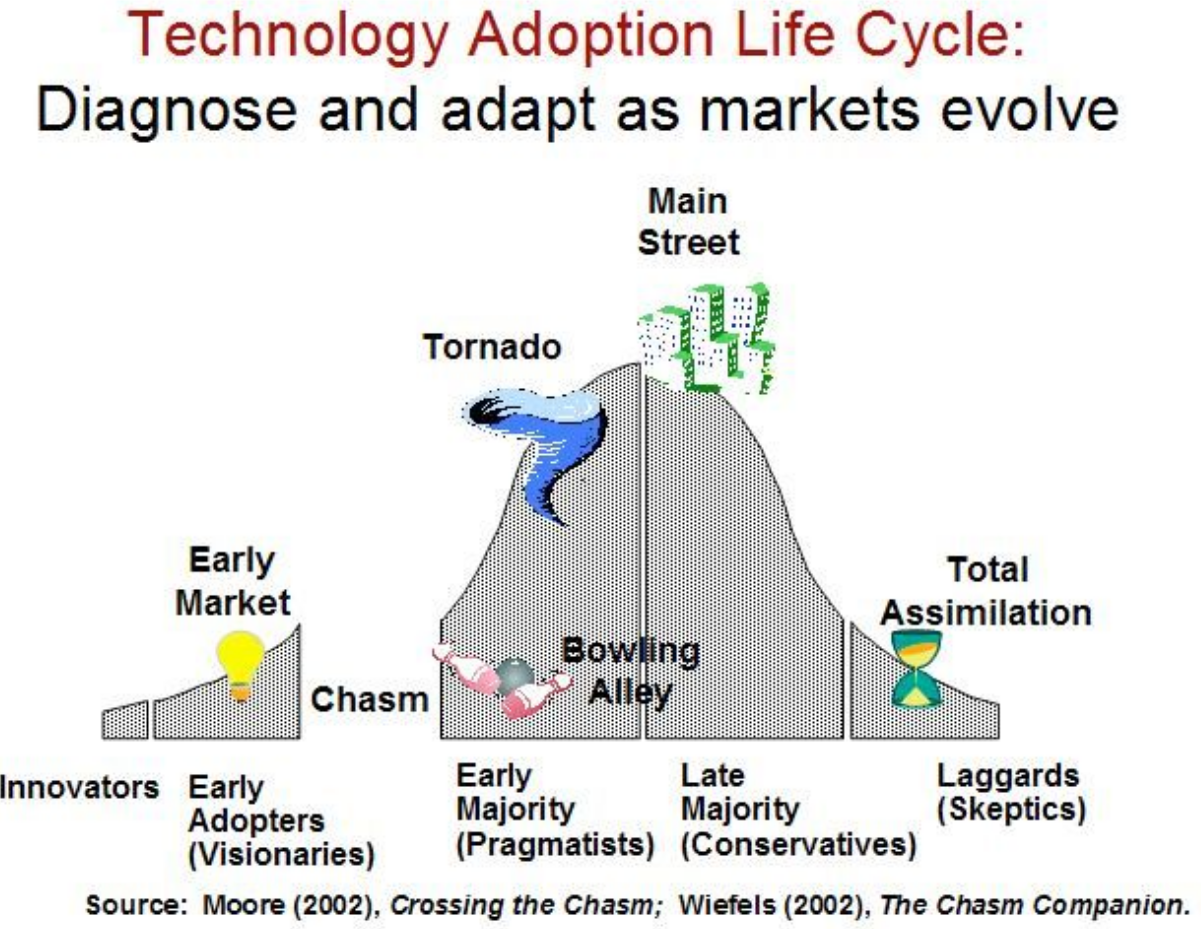
\includegraphics[scale=0.3]{images/Markadopters.png}
	\caption{Pensiero Capitalista}
	\label{fig:cap}
\end{figure} 

\subsection{Cosa può influenzare percezioni e aspettative del mercato?}
La strategia dell’annuncio
\begin{itemize}
	\item Può creare nel mercato una percezione della base di installazioni più
	ampia della realtà
	\item Può aumentare la quota di “ricordo” tra i potenziali clienti ( share of mind)
	\item Può convincere i clienti a rinviare l’acquisto del prodotto di un
	concorrente
	\item La reputazione dell’impresa
	\item Esercita un influenza decisiva circa le probabilità di successo del nuovo
	prodotto
	\item L’irreversibilità degli impegni strategici
	\item Per dimostrare il proprio impegno in un determinato settore l’impresa può
	effettuare ingenti investimenti difficilmente reversibili
	
\end{itemize}


\section{Strategie di innovazione nelle PMI}
L’innovazione non è una dimensione esclusiva delle grandi imprese o una
prerogativa delle aziende che operano nei settori high-tech.
Innovare è un sentiero decisivo e percorribile anche per le \textbf{piccole imprese},
anche per chi agisce in mercati tradizionali.
L’innovazione è una delle leve fondamentali che una piccola impresa può
azionare per intraprendere un percorso di crescita o rafforzare la sua
strategia di \textbf{differenziazione focalizzata}.
A fronte dei vincoli di risorse finanziarie e manageriali, una piccola
impresa innovativa talvolta mostra di essere\textbf{ più agile e più rapida}
nell’adattamento ai cambiamenti dello scenario competitivo.
Fondamentali sono il ruolo dell’imprenditore e la capacità di
stabilire relazioni con altri attori dell’ecosistema dell’innovazione.

\subsection{Una popolazione eterogenea}
Il mondo delle piccole imprese è popolato da “abitanti” con profili e
comportamenti molto differenti: accanto ad aziende con elevate
competenze tecnologiche, convivono aziende appartenenti a settori
tradizionali, dove sovente l’innovazione ha un carattere informale e si
concentra sul marketing e l’organizzazione, rimanendo “invisibile” e
nascosta alle rilevazioni statistiche.

Per gli imprenditori italiani è soprattutto il deficit di risorse finanziarie la
barriera di maggior impatto percepita tra gli ostacoli che intralciano i processi
di innovazione.

Le attività innovative hanno luogo in modi molto diversi nelle industrie. Si può
osservare una forte concentrazione di attività tecnlogiche in pochi innovatori e,
nello stesso tempo, in un’altro settore industrial, all’interno della popolazione
d’imprese, una grande distribuzione di attività innovative.
In alcuni settori, le grandi imprese svolgono un ruolo fondamentale per
l’innovazione mentre, in altri, le piccolo imprese risultano particolarmente attive.
In alternativa, gli innovatori possono rimanere nel loro ruolo per un lungo period
oppure possono trovarsi di fronte ad una profonda turbolenza nelle attività
innovative ed essere superati da nuovi entrant.
In poche parole, le attività innovative mostrano percorsi organizzativi molto
diversi nei diversi settori industriali.
.
Gli elementi endogeni della dinamica industrial sono la dimensione d’impresa, la
struttrua di mercato e l’innovazione (proprietà della tecnologia e processo di
apprendimento)

\subsection{Ruolo dell'imprenditore e i regimi tecnologici}


\begin{figure}[h!]
	\centering
	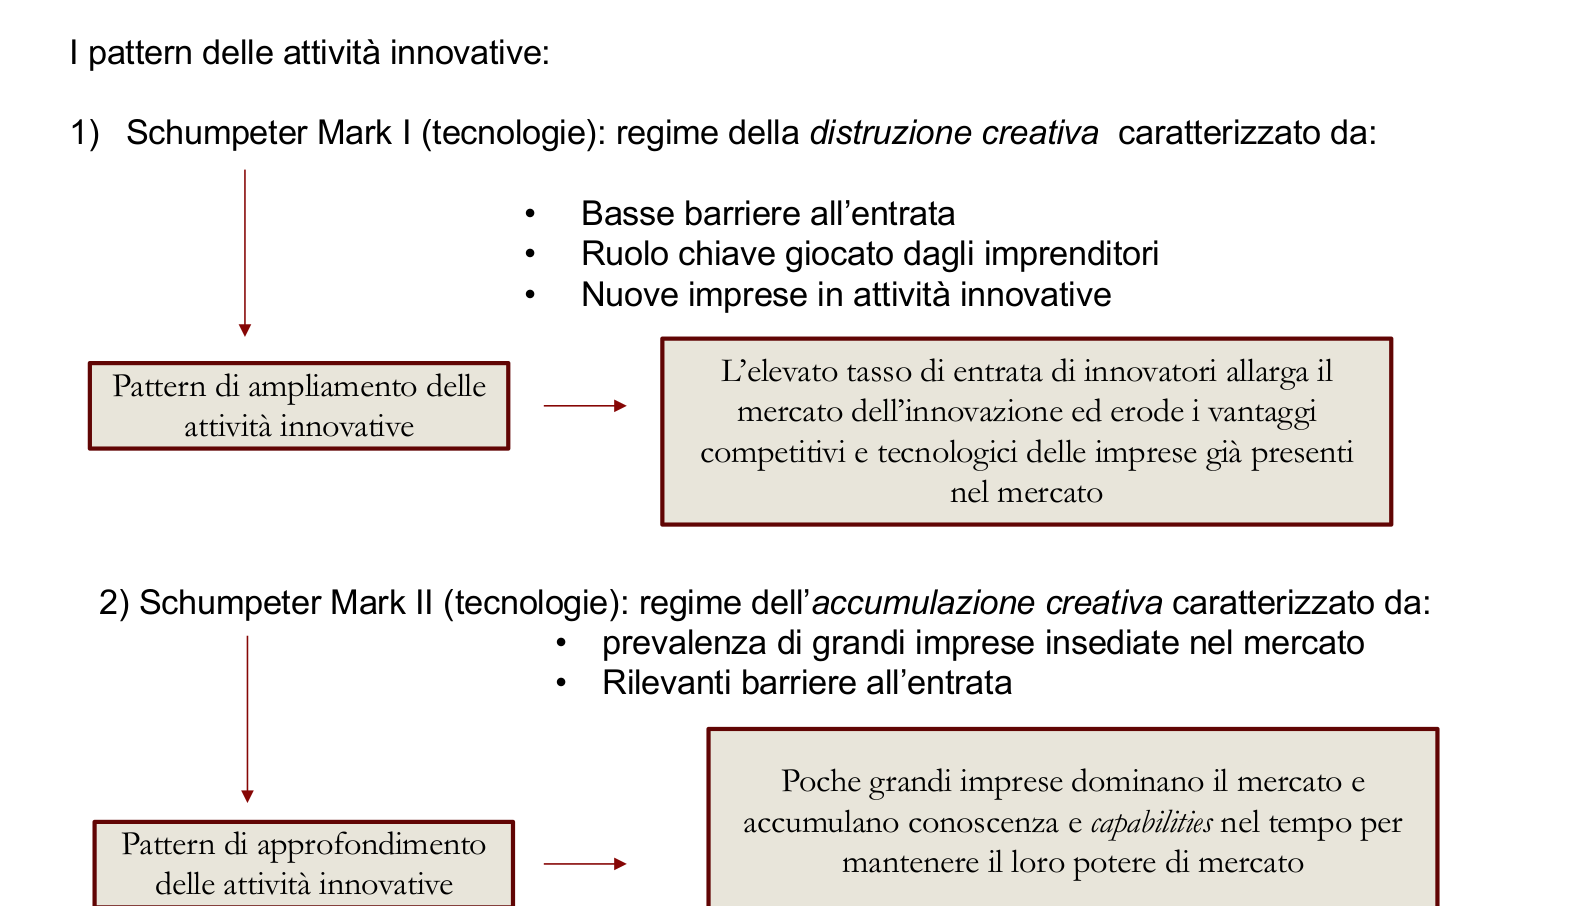
\includegraphics[scale=0.3]{images/ruoloimp.png}
	\caption{Ruolo dell'impredntiore}
	\label{fig:imp}
\end{figure} 

\subsection{Imprenditore orientato all'innovazione}
Un imprenditore orientato all’innovazione dovrà essere capace di
assolvere alcuni fondamentali compiti.
\begin{itemize}
	\item Attirare e trattenere in azienda gli “innovatori”
	\item Elaborare una visione dei processi innovativi chiara e condivisa
	nell’organizzazione
	\item Determinare la rotta da seguire per raggiungere gli obiettivi fissati verso cui far
	convergere le energie dell’azienda
	\item Accettare il rischio di sostenere nuove idee, anche se contrastanti con il
	disegno strategico originario
	\item Selezionare e guidare squadre con talenti “complementari”
	\item Diffondere e consolidare nell’azienda una cultura dell’innovazione
\end{itemize}


Per la maggior parte delle piccole imprese, l’innovazione è un processo
graduale, basato sull’ascolto e la risoluzione di problemi dei clienti, di
adattamento costante e tempestivo alle mutevoli esigenze della domanda.
Non mancano, però, i casi di innovazione radicale, soprattutto nelle fasi
embrionali di nuovi settori o di discontinuità tecnologica.
Il divario che le piccole imprese sono costrette a scontare in termini di
differenziale di risorse con le aziende maggiori tende ad assottigliarsi quando
riescono a dotarsi di flessibilità organizzativa, rapidità di reazione, capacità di
personalizzazione dei prodotti, innovazione ad hoc.

\subsection{Le fonti dell'innovazione }
Le piccole imprese possono beneficiare di una molteplicità di fonti per
intraprendere processi innovativi, soprattutto se dotate di capacità relazionali:
clienti ,fornitori ,università e istituzioni di ricerca ,cluster e distretti concorrenti e complementor.

\subsection{Competenze relazionali}
Per trarre vantaggio da una collaborazione per lo
sviluppo innovativo, è fondamentale saper
selezionare un partner.
Soprattutto quando il partner è una grande
impresa, la piccola impresa dovrà sviluppare
competenze relazionali e capacità negoziali per
evitare di essere “svuotata” delle sue conoscenze
e non rischiare di soccombere, schiacciata dal
potere contrattuale del partner.


\subsection{Spin-off Accademici}
Gli spin-off sono piccole imprese innovative che traggono origine dai laboratori
di università e centri di ricerca.
Gli spin-off sono considerati tra le modalità più efficaci per favorire il
trasferimento dei risultati della ricerca verso il sistema industriale.
In relazione alle determinanti dei processi di spin-off, la letteratura distingue tra
variabili “macro”, “meso” e “micro”.
\begin{itemize}
	\item MICRO – riguardano i tratti personale del ricercatore che aspira a diventare
	imprenditore e i caratteri strutturali e organizzativi dell’impresa nascente.
	\item MESO – riflettono le caratteristiche dell’istituzione di provenienza, nonché le
	politiche e gli strumenti di valorizzazione della ricerca e a sostegno del
	trasferimento tecnologico.
	\item MACRO – rappresentano i fattori legati all’ambiente esterno e in grado di
	condizionare le scelte strategiche e le performance dell’impresa spin-off.
\end{itemize}

Un fattore decisivo per gli spin-off è l’ambiente innovativo che li circonda: le
risorse tangibili e intangibili del territorio, la rete di relazioni, la domanda delle
imprese, la presenza di capitale di rischio, l’azione di strumenti e policy pubbliche,
concorrono a creare un ecosistema dell’innovazione da cui lo spin-off attinge gli
ingredienti essenziali per il suo percorso iniziale.
\subsection{Processi di Trasferimento Tech.}
Il processo di trasferimento di tecnologie e conoscenze dal mondo della ricerca
verso le piccole e medie imprese non è di semplice realizzazione.
Sovente, è molto difficile riuscire a cogliere con precisione la domanda di
innovazione che proviene dalle aziende; inoltre, molte imprese di piccole
dimensioni non dispongono di un’adeguata capacità di assorbimento.

In letteratura, le criticità del processo di trasferimento sono
distinte in problemi dal lato della domanda (demand-side) e dal lato
dell’offerta (supply-side).


\begin{figure}[h!]
	\centering
	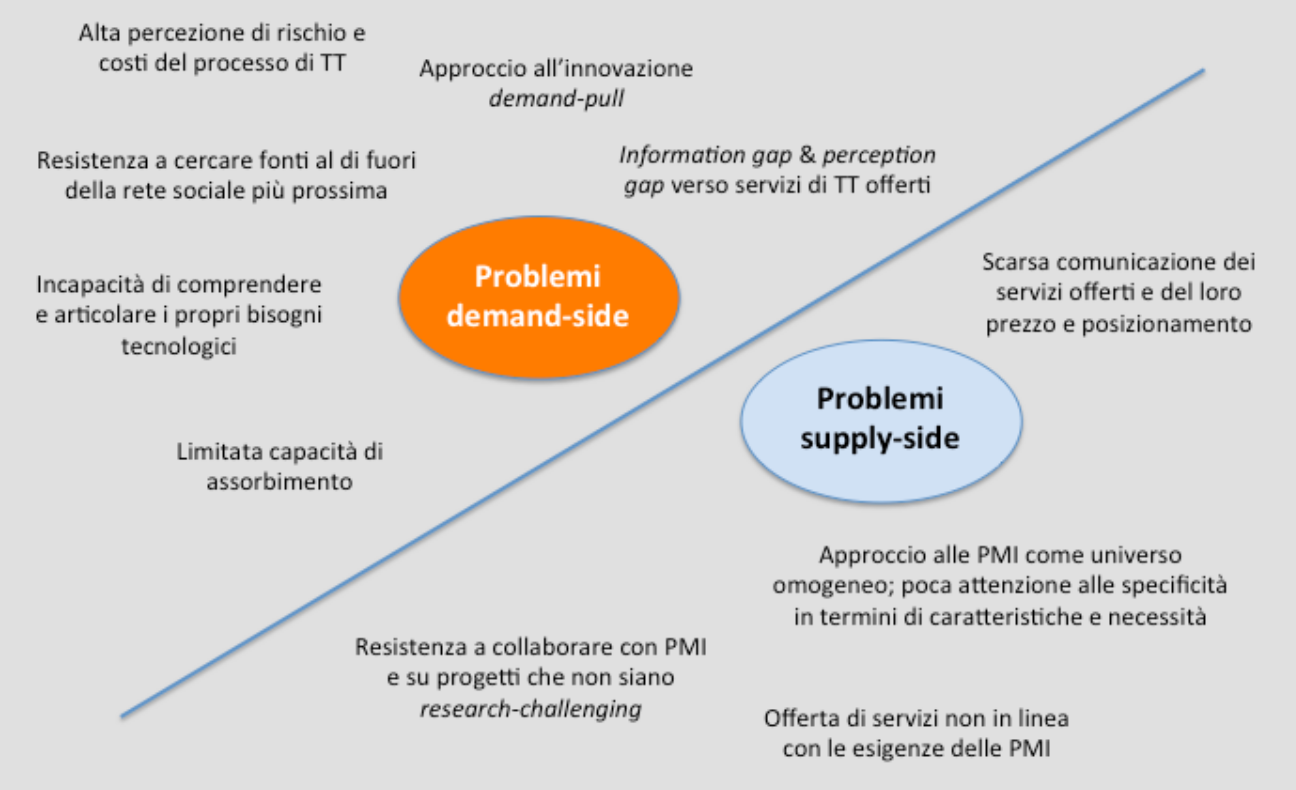
\includegraphics[scale=0.3]{images/ttf.png}
	\caption{Trasferimento Tech.}
	\label{fig:ttf}
\end{figure} 


\subsection{Forme dell'innovazione}
Flessibilità organizzativa e capacità di personalizzazione,
innovazione ad hoc e rapidità di adattamento sono esaltate nelle
nuove forme di “artigianato digitale”, rese possibili
dall’evoluzione delle tecnologie.
Le nuove tecnologie aprono spazi di mercati per le piccole
imprese alla ricerca di sbocchi commerciali e di partnership per lo
sviluppo dell’innovazione e desiderose di rintracciare competenze
non possedute, consentendo anche alle PMI di adottare modelli di
open innovation.


\section{I sistemi di Innovazione Nazionale }
l successo di questo concetto è legato al fallimento dell’economia
mainstream nel comprendere quali sono i fattori rilevanti nella
competition internazionale.
Il SIN si basa sull’architettura dei flussi di conoscenza poiché le
attività economiche sono sempre più knowledge-intensive, e gli
investimenti in conoscenza richiedono R\&S, livelli superiori di
formazione e di training nel lavoro creativo.

L’approccio del SIN identifica quattro flussi fondamentali di conoscenza
tra gli attori dell’innovazione:
\begin{itemize}
	\item Interazione tra imprese
	\item Interazione tra imprese, università e laboratory pubblici di ricercar
	\item Diffusione di conoscenza e tecnologie alle imprese
	\item Movimenti del personale
	\item L’interazione e il coinvolgimento delle istituzioni è cruciale per stimolare
	l’apprendimento.
	\item Le istituzioni sono il fattore principale perché rapprensentano le norme,
	le abitudini e le regole che influenzano il modo in cui le persone si
	relazionano e utilizzano la conoscenza
\end{itemize}

I vettori istituzionali che hanno un maggior impatto sulle differenze
nazionali dei sistemi d’innovazione sono:
\begin{enumerate}
	\item L’orizzonte temporale degli agenti
	\item Il ruolo della fiducia
	\item Il mix attuale di razionalità
\end{enumerate}

L’impianto teorico normalmente utilizzato per studiare il SIN è basato su
due dimensioni:
La struttura del Sistema
\begin{itemize}
	\item Cosa viene prodotto nel Sistema economico?
	\item Quali competenze sono più sviluppate?
\end{itemize}
L’organizzazione istituzionale
In che modo produzione, innovazione e apprendimento avvengono?

\subsection{Le fonti della conoscenza}
l’interazione tra le imprese
\textbf{Interazione cliente-fornitore}
\begin{itemize}
	\item Innovazione per accumulazione di conoscenza
	\item Allineamento cognitive
	\item Interazioni di apprendimento attraverso relazioni stabili
	(codici comuni di comunicazione)
	\item  Bassi costi di transazione
	
\end{itemize}

\textbf{Fattori nazionali specifici}
\begin{itemize}
	\item Reti locali di imprese innovative
	\item Clienti (imprese) molto competenti
\end{itemize}

\textbf{Interazioni Orizzontali}
\begin{itemize}
	\item Cooperazione tecnologica e creazione di reti d’imprese
	\item  Organizzazioni reticolari e diffusione della conoscenza
\end{itemize}


\textbf{Ricerca Scientifica  e Sistema d'Istruzione }
\begin{itemize}
	\item L’Università influisce sulla capacità d’innovazione in tre modi diversi:
	
	\item Offre una cultura generale che facilita la decodifica del mondo
	reale e delle sue dinamiche (problem-solving capacity)
	\item Crea competenze specifiche (abilità tecniche)
	\item Produce laboratori di ricerca
	\item La ricercar scientifica è anche prodotta in centri di ricercar
	dedicati allo “spostamento in avanti” della frontiera tecnologica
	per le imprese
	\item  Organizzazioni reticolari e diffusione della conoscenza
\end{itemize}
Il ruolo del Sistema d’Istruzione gioca un ruolo cruciale nei SIN

\textbf{Il sistema Finanziario}
Le istituzioni finanziarie devono sviluppare la capacità di valutare e selezionare
proposte di investimento in R\&S sulla base dei ricavi attesi. Quali sono I
problem che devono affrontare?
L’agente finanziario possiede informazione incompleta rispetto alla funzione
obiettivo del manager e anche rispetto alle sue azioni e ai relative effetti attesi
(potrebbe registrare un fallimento. Si pone il problema del controllo del
manager).
Un’informazione incomplete produce problem di selezione avversa e problemi
d’incentivazione (azzardo morale). Il risultato di questo deficit informative porta
ad un investimento subottimale anche per quegli investimenti con un valore
netto di sconto postivo.

\textbf{La politica tecnologica e il ruolo del governo}
Le strategie tecnologiche
nazionali influenzano le
performance innovative delle
imprese perchè sostengono lo
sviluppo di una specifica
tecnologia e attraverso questa
azione sostengono e promuovo il
cambiamento tecnologico.
Normalmente, nel paesi OECD, I
governi sostengono 1/3 della
spesa totale in R\&S.

\section{Il ruolo della Conoscenza }
Quali sono le condizioni che definiscono se un sistema economic è basato
sulla conoscenza?
Per rispondere dobbiamo spiegare il meccanismo fi evoluzione della
conoscenza e perchè questo meccanismo può essere considerato una
forza trainantedella competitività.

La produzione, organizzazione e controllo della conoscenza è una
caratteristica tipica delle società capitalistiche. Come affermava Schumpeter,
la dinamica dell’innovazione disturba il meccanismo di mercato.
E questo disequilibrio produce:


\begin{figure}[h!]
	\centering
	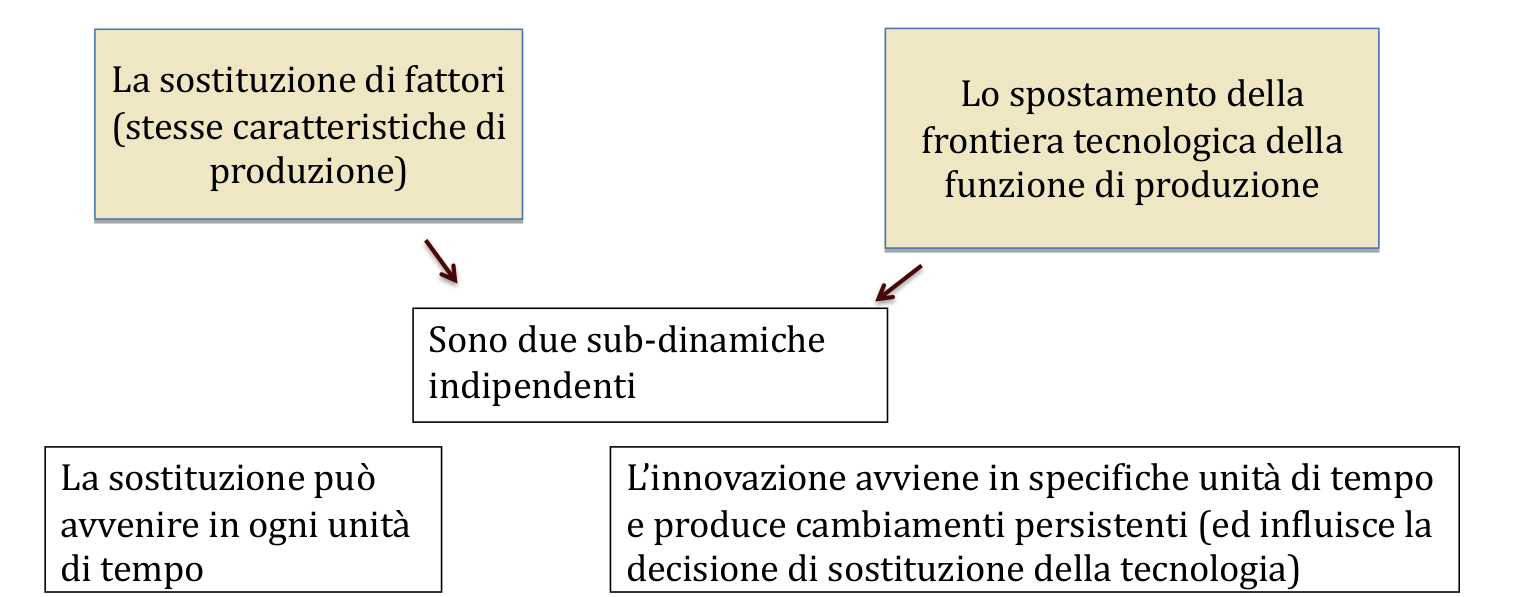
\includegraphics[scale=0.3]{images/dinInn.png}
	\caption{Dimensione Inovnazione SIN}
	\label{fig:Dim}
\end{figure} 




L’innovazione implica anche l’esistenza di una capacità di gestire gli
obiettivi del Sistema socio-economic. In altri termini, di saper
organizzare la conoscenza.
Dato che l’innovazione è:
\begin{itemize}
	\item Place-specific
	\item Dipende dalla relazioni di scambio (bottom-up, top-down)
	\item  È legata al sistema di produzione di nuove idee (nuove soluzioni)
\end{itemize}

Possiamo osservare una diversa intensità nell’interazione delle sub-
dinamiche perchè queste non sono coordinate ex-ante e perchè sono
influenzate dalla loro co-evoluzione (lock-in, disruptive innovation, ...).

\subsection{Il modello delal triplice elica}
It describes the knowledge infrastructure in terms of overlapping
institutional spheres, with each taking the role of the other and with hybrid
organizations emerging in the interfaces.
The aim of this model is to realize an innovative environment
consisting of university spin-off, tri-lateral initiatives for knowledge-
based economic development and strategic alliances among firms (large
and small, operating in different areas and with different levels of
technology), government laboratories and academic research groups.
These arrangements are often encouraged, but not controlled, by
government, whether through new “rules of the game” direct or
indirect financial assistance.
(Etzkowitz, H., L. Leydesdorff, 2000)

Il concetto della Triplice Elica si presenta come un’evoluzione del SIN
nel senso che quest’ultimo integra produzione e innovazione a livello
Nazionale mentre nell’economia globalizzata, l’innovazione genera
diversi effetti istituzionali e geografici.
Questo significa che l’analisi del SIN deve tenere in considerazione tre
sub-dinamiche:

\begin{figure}[h!]
	\centering
	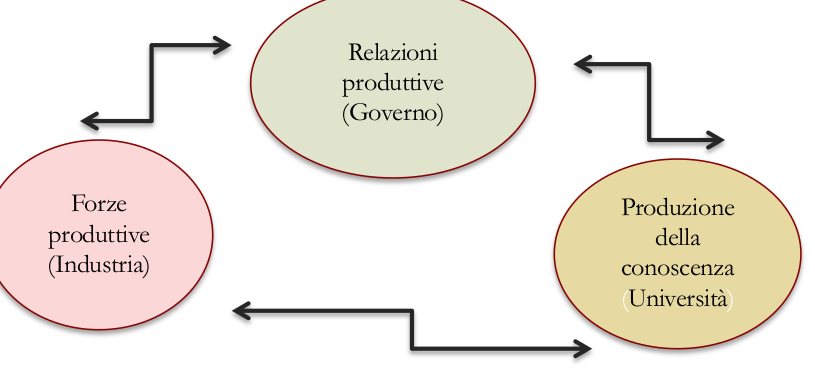
\includegraphics[scale=0.3]{images/SIN.png}
	\caption{Trasferimento Tech.}
	\label{fig:ttf}
\end{figure} 

Le relazioni Università-Industria-Governo ri-combinano tre funzioni
fondamentali di un Sistema socio-economico:
\begin{itemize}
	\item Produzione e conservazione della ricchezza
	\item Produzione di novità (nuova conoscenza)
	\item Controllo delle interface delle sub-dinamiche del Sistema
\end{itemize}

Come? Attraverso due livelli di interazione
\begin{itemize}
	\item 1mo livello: ogni istituzione vincola il comportamento delle altre due
	\item 2ndo livello: ogni istituzione possiede relazioni in grado di influenzare le
	aspettative degli altri due attori. 
\end{itemize}

Le tre funzioni obiettivo devono
ricombinarsi al fine di:
\begin{itemize}
	\item	produrre ricchezza
	\item Produrre novità in capo scientifico e tecnologico
	\item Garantire la sostenibilità e ri-producibilità del Sistema socio-
	economico.
\end{itemize}


\section{IL Caso Netflix}


\end{document}
